\documentclass[12pt]{report}
\usepackage{hyperref}
\usepackage{gensymb}
\usepackage{imakeidx}
\usepackage{amsmath}
\usepackage{listings}
\usepackage{graphicx}
\usepackage{sidecap}
\usepackage{pgfplots}
\usepackage{caption}
\usepackage{subcaption}
\usepackage{footnote}
\makesavenoteenv{tabular}
\pgfplotsset{compat=1.9}
\graphicspath{ {./Images/} }

\makeindex

\begin{document}
\title{Modeling Low Earth Orbit Constellations for Networking}
\author{Joseph McGuchan}
\maketitle
\thispagestyle{empty}

%TODO Cover Sheet



%TODO Declaration of Originality

\chapter{Declaration of Originality}

I, Joseph Law McGuchan of King's College, being a candidate for Part II of the Computer Science Tripos, hereby declare that this dissertation and the work described in it are my own work, unaided except as may be specified below, and that the dissertation does not contain material that has already been used to any substantial extent for a comparable purpose.

Signed %TODO

Date %TODO

\chapter{Proforma}

%TODO Proforma

%Your candidate number.
%The Title of your Project. 
Modeling Low Earth Orbit Constellations for Networking
%The Examination and Year.
%Word-count for the dissertation.
%Final line count: Number of lines written by the *student* in the final version of their %software work.
%Project Originator.
%Project Supervisor.
%At most 100 words describing the original aims of the project.
%At most 100 words summarizing the work completed.
%At most 100 words describing any special difficulties that you faced. 
%(In most cases the special difficulties entry will say “None”.)

\tableofcontents

%==============================================================================================================================
%----------------------------------------------------------------------------------------------------------INTRODUCTION-------------------------------------------------------------------------------------------------------
%==============================================================================================================================
\chapter{Introduction}

SpaceX are planning to launch a constellation of thousands of low Earth orbit (LEO) communication satellites in the next few years. The objective of this constellation, called Starlink, is to provide low-latency internet connection across the world.

The satellites in this network will be in constant motion, not just relative to the ground, but relative to one another, creating a network with a constantly changing topology and associated latencies. The question of how to structure such a network, and what the resultant latencies of said network will be, has not been thoroughly explored, but it will become increasingly relevant as more and more companies build similar constellations. If these Constellations prove to provide significant gains in latency while providing competitive bandwidth, they might render previous submarine optical cables obsolete.

My goals are:
\begin{enumerate}
	\item To create visualizations of the SpaceX constellation.
	\item To experiment with different topologies of the SpaceX network and test their associated latencies. 
\end{enumerate}

%============================================WHAT IS STARLINK======================================================
\section{What is Starlink?}

The purpose of Starlink is to provide low latency internet connections, as of 17/05/19, there are two companies offering satellite internet services, Excede\cite{ExcedeWebsite}, and Hughes, whose 9202 BGAN Land Portable Satellite Terminal offers connection speeds up to 464kbps\cite{HughesWebsite}. These companies largely target domestic use in rural areas which don’t have a faster coverage, and corporations, providing internet connections to airplanes and cargo ships. Currently, Satellite Internet connection is a last resort, something turned to when conventional means of connection are not available, Starlink intends to invert this, turning satellite internet into the premium option. 

The difference between Starlink and currently existing brands is that current brands use geostationary satellites \cite{HughesPressRelease}, while Starlink will use LEO satellites. The significantly shorter distance will create much shorter paths for signals. On top of this, SpaceX will be utilizing laser communication between satellites, as opposed to the competitors who have little to no intra-satellite communication. In the vacuum of space, light travels 47\% faster than in glass \cite{PropertiesOfGlass}. Therefore, in theory, a LEO network utilizing lasers would achieve latencies far lower than that by even the best terrestrial fiber optic connections over long distances.

%============================================WHY FOCUS ON STARLINK======================================================
\section{Why Focus on Starlink?}

Starlink is only one of a number of different LEO internet networks that have been proposed, so why should I focus on it's topology? Ideally, I would like the conclusions of my study to be generalized to many other LEO constellations. However, constellations are approved by the FCC on a case-by-case basis, using a complicated and changing system of legislation, it's not easy to know what a normal network looks like. By analyzing the properties of a network of my own design, I run a much greater risk of coming to conclusions that cannot be generalized, as I am not working on an FCC-approved constellation. By analyzing the properties of Starlink, we are analyzing a network that is confirmed legally and scientifically plausible.

But there is another reason to investigate Starlink. As the largest of most high-profile attempts to build a LEO internet backbone, Starlink represents the most significant competitor to other emerging satellite communications networks and the one more likely to become dominant in future years. By theorizing about it's properties now, we can prepare ourselves for the changes Starlink might pose to communications in the upcoming years.

%============================================WHY CREATE A VISUALISATION======================================================
\section{Why Create a Visualisation?}
When it comes to understanding a network such as Starlink, a visual description is incredibly valuable. By visualizing the network we can develop an intuition for how it operates, and use that intuition to develop ideas for new algorithms and structures for testing.

Creating a visualization also poses a minimal additional cost on my part, as to accurately model the latencies between base stations I will need to simulate satellite positions and links anyway.

%============================================MARK HANDLEY'S WORK======================================================
\section{Mark Handley's Work}

My initial proposal for the project was inspired by the findings of an existing study done by Mark Handley, since proposing the project, Mark Handley has made his results publicly available \cite{OriginalReport}, so my new goal will be to replicate and expand upon his findings.

%============================================WHAT I WILL BE USING======================================================
\section{What I Will Be Using}
To create the visualization I will be using the open-source game engine Godot. Using a game engine struck me as the simplest way to create a visualization tool, and Godot, being powerful, open-source, and capable of running easily on many devices, seemed like the ideal choice.

For the parts of code related to visualization I will be using Godot's build in script GDScript, which is easy to use and specifically designed to integrate well with the Godot engine. For parts of the code related to simulation I will use C\#, which Godot is compatible with, and which offers significance performance improvements over GDScript.

%============================================EXAMPLE OF RESULTS======================================================
\section{Example of Results}
To give an example of my program at work I have included a few screenshots seen in figure \ref{fig:Screenshots}. The program that I created is capable to simulating different linking methods between satellites, different rates of satellite failure, and performing a number of tests including highlighting the shortest path between two nodes. In all the images the red line is the shortest path between the two spherical base stations, while the gray lines represent available links.

\begin{figure}
	\centering
	\caption{Screenshots of my program simulating the shortest path between two nodes through different linking methods and rates of satellite failure, the highlighted path is the shortest path between the two base stations.}
	\label{fig:Screenshots}
	\begin{subfigure}[b]{\textwidth}
		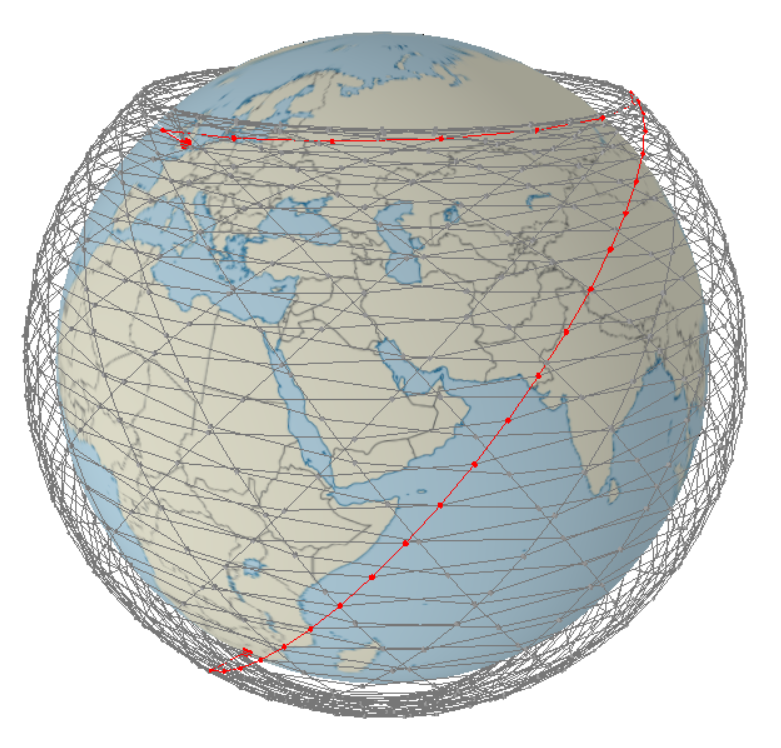
\includegraphics[width=\textwidth]{LDN-JHB-H0-1}
	\end{subfigure}
	
	\begin{subfigure}[b]{0.4\textwidth}
		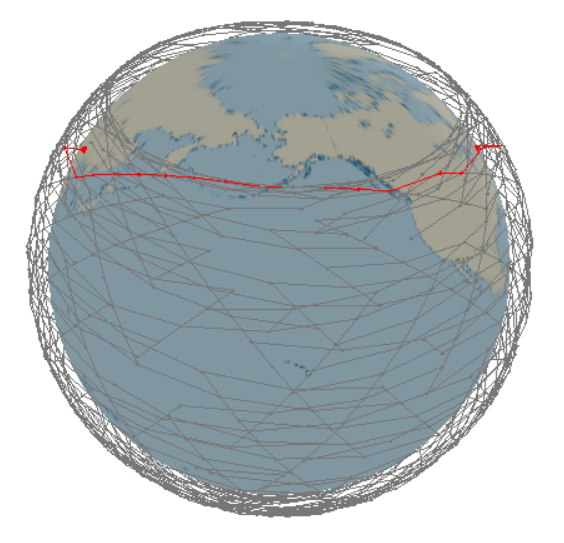
\includegraphics[width=\textwidth]{NewYorkBeijing1320SatellitesLM2}
	\end{subfigure}
	\hfill
	\begin{subfigure}[b]{0.4\textwidth}
		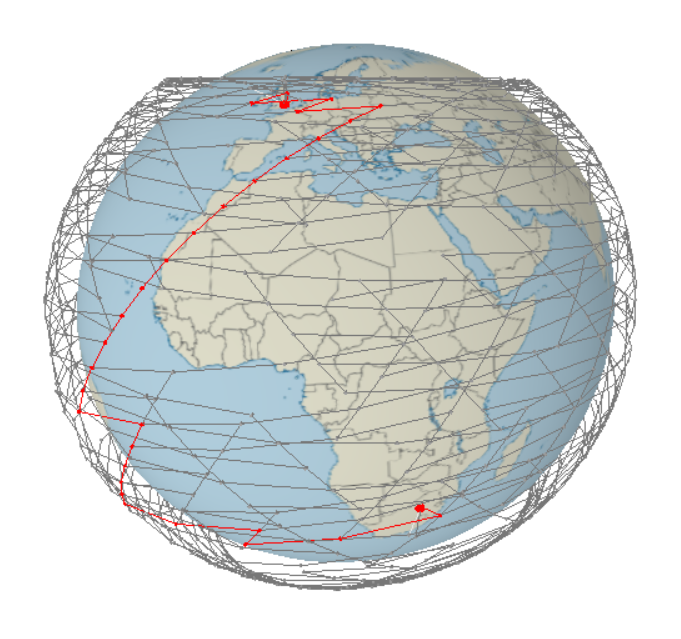
\includegraphics[width=\textwidth]{LondonJohannasburg1254SatellitesLM2}
	\end{subfigure}
\end{figure}

%============================================CURRENT STATE OF EVENTS======================================================
\section{Current State of Events}
As of May 11th 2019, SpaceX have loaded their first 60 satellites into their Falcon rocket, and are preparing to launch them \cite{ElonMuskTweet2}. This report is therefore being released at the optimal time for researchers hoping to get ahead of what could potentially be the next revolution in internet communications.

%==============================================================================================================================
%----------------------------------------------------------------------------------------------------------PREPARATION---------------------------------------------------------------------------------------------------------
%==============================================================================================================================
\chapter{Preparation}

%============================================STARING POINT======================================================
\section{Starting Point}

Most of the information I will be using for the structure of the SpaceX network comes from their application to the FCC on March 29th, 2018\cite{FCCApplication}, and their technical attachment\cite{TechnicalAttachment}, which outlines the various orbital spheres, planes within each sphere, and various other details of the constellation. I will also be building on insights gleaned from Handley's original research. The insights that I will be building off of are:

\begin{enumerate}
\item The optimum phase offset is 9/33.
\item Satellites will most likely link to those moving in the same direction as them.
\item Starlink will most likely use a static routing method, and it is therefore most important to examine the shortest paths between two points in the network.
\end{enumerate}

These insights will be returned to throughout my report and explanations will be given as to exactly what these insights mean.

SpaceX have already sent up two test satellites, and according the Elon Musk, they are working very well, providing a latency of only 25ms\cite{ElonMuskTweet}.

%============================================THE STRUCTURE OF STARLINK======================================================
\section{The Structure of Starlink}

There is a lot we do not know about Starlink, but this is what we can infer from SpaceX’s application to the FCC\cite{FCCApplication}, 

Starlink was initially going to be a constellation of 4,425 LEO satellites. The initial proposal to the FCC came in the form outlined in figure \ref{fig:Starlink Orbits}, however Starlink have since changed their proposed satellite constellation\cite{StarlinkChange}. It is as of yet unclear what structure the completed Starlink network will have, but we do know what the first sphere's properties will be (given in figure \ref{fig:Starlink Within Program}).

\begin{figure}
\begin{center}
\caption{The layout of Starlink initially proposed}
\label{fig:Starlink Orbits}
\begin{tabular}{|c|c|c|c|c|c|}
\hline
\multicolumn{6}{|c|}{SPACEX SYSTEM CONSTELLATION} \\
\hline
Parameter & Initial Deployment & \multicolumn{4}{|c|}{Final Deployment} \\
& (1,600 satellites) & \multicolumn{4}{|c|}{(2,825 satellites)} \\
\hline
Orbital Planes & 32 & 32 & 8 & 5 & 6 \\
Satellite per Plane & 50 & 50 & 50 & 75 & 75 \\
Altitude & 1150km & 1110km & 1130km & 1275km & 1325km \\
Inclination & 53\degree & 53.8\degree & 74\degree & 80\degree & 70\degree \\
\hline
\end{tabular}
\end{center}
\end{figure}

In it's application to the FCC SpaceX was required to state any notable debris that might not burn up if a satellite were to descend from orbit. Among the components listed where 5 silicon carbide “communication components”, silicon carbide is used in mirrors for laser communication links, and we can therefore conclude that SpaceX's satellites will have, at most, 5 available links to form with nearby satellites.

We also know information about how Starlink satellites will communicate with ground stations, a base station may only connect with a satellite at an inclination less than 40\degree from the vertical using Radio Frequency (not laser) connections. Connections will be stronger to satellites directly overhead, however as Starlink does not provide much information in exactly how their intra-satellite communications work, speculations on bandwidth will not prove to be helpful.

%============================================MODELLING SATELLITES IN ORBIT======================================================
\section{Modeling Satellites in Orbit}

The position of a satellite above the surface of the earth can be described by 4 values. \cite{Book}

 \begin{description}
\item[Altitude]
\item[Inclination]
This is the angle between the orbital plane, and the equatorial plane, (the plane on which the equator lies).
\item[Longitudinal Offset]
If inclination is greater than 0\degree, then the orbital plane and equatorial plane will intersect at a line, the angle between this line and the plane described by the great circle at longitude 0\degree is the longitudinal offset. In other words, the Longitudinal offset is the Longitude of the point where this line passes through the surface of the earth.
\item[True Anomaly]
The angle between the line drawn from the origin to the satellite, and the line drawn from the origin to the point on the satellite's orbit of longitude 0.
\end{description}

To better visualize this, figure \ref{Describing an orbit} describes how would would calculate the position of a satellite in space from these four values.

\begin{enumerate}
\item First, take the orbit around the equator of the chosen altitude. Place your satellite so that it is directly above the position with terrestrial coordinates (0,0).
\item Now, look at the earth from the side, so that your satellite is as far to the right of your view as possible, and the orbit it is on is flat. Tilt to the orbit until it's angle to the equator is equal to the inclination.
\item Now return to looking down on the earth from above, and rotate the orbit by your longitudinal offset clockwise.
\item Finally move so that the orbit forms a flat circle in your view, rotate the satellite clockwise around it's orbit by the true anomaly.
\end{enumerate}

\begin{figure}
	\caption{How to calculate the location of a satellite from it's Altitude, Inclination, Longitudinal Offset and True Anomaly}
	\label{Describing an orbit}
	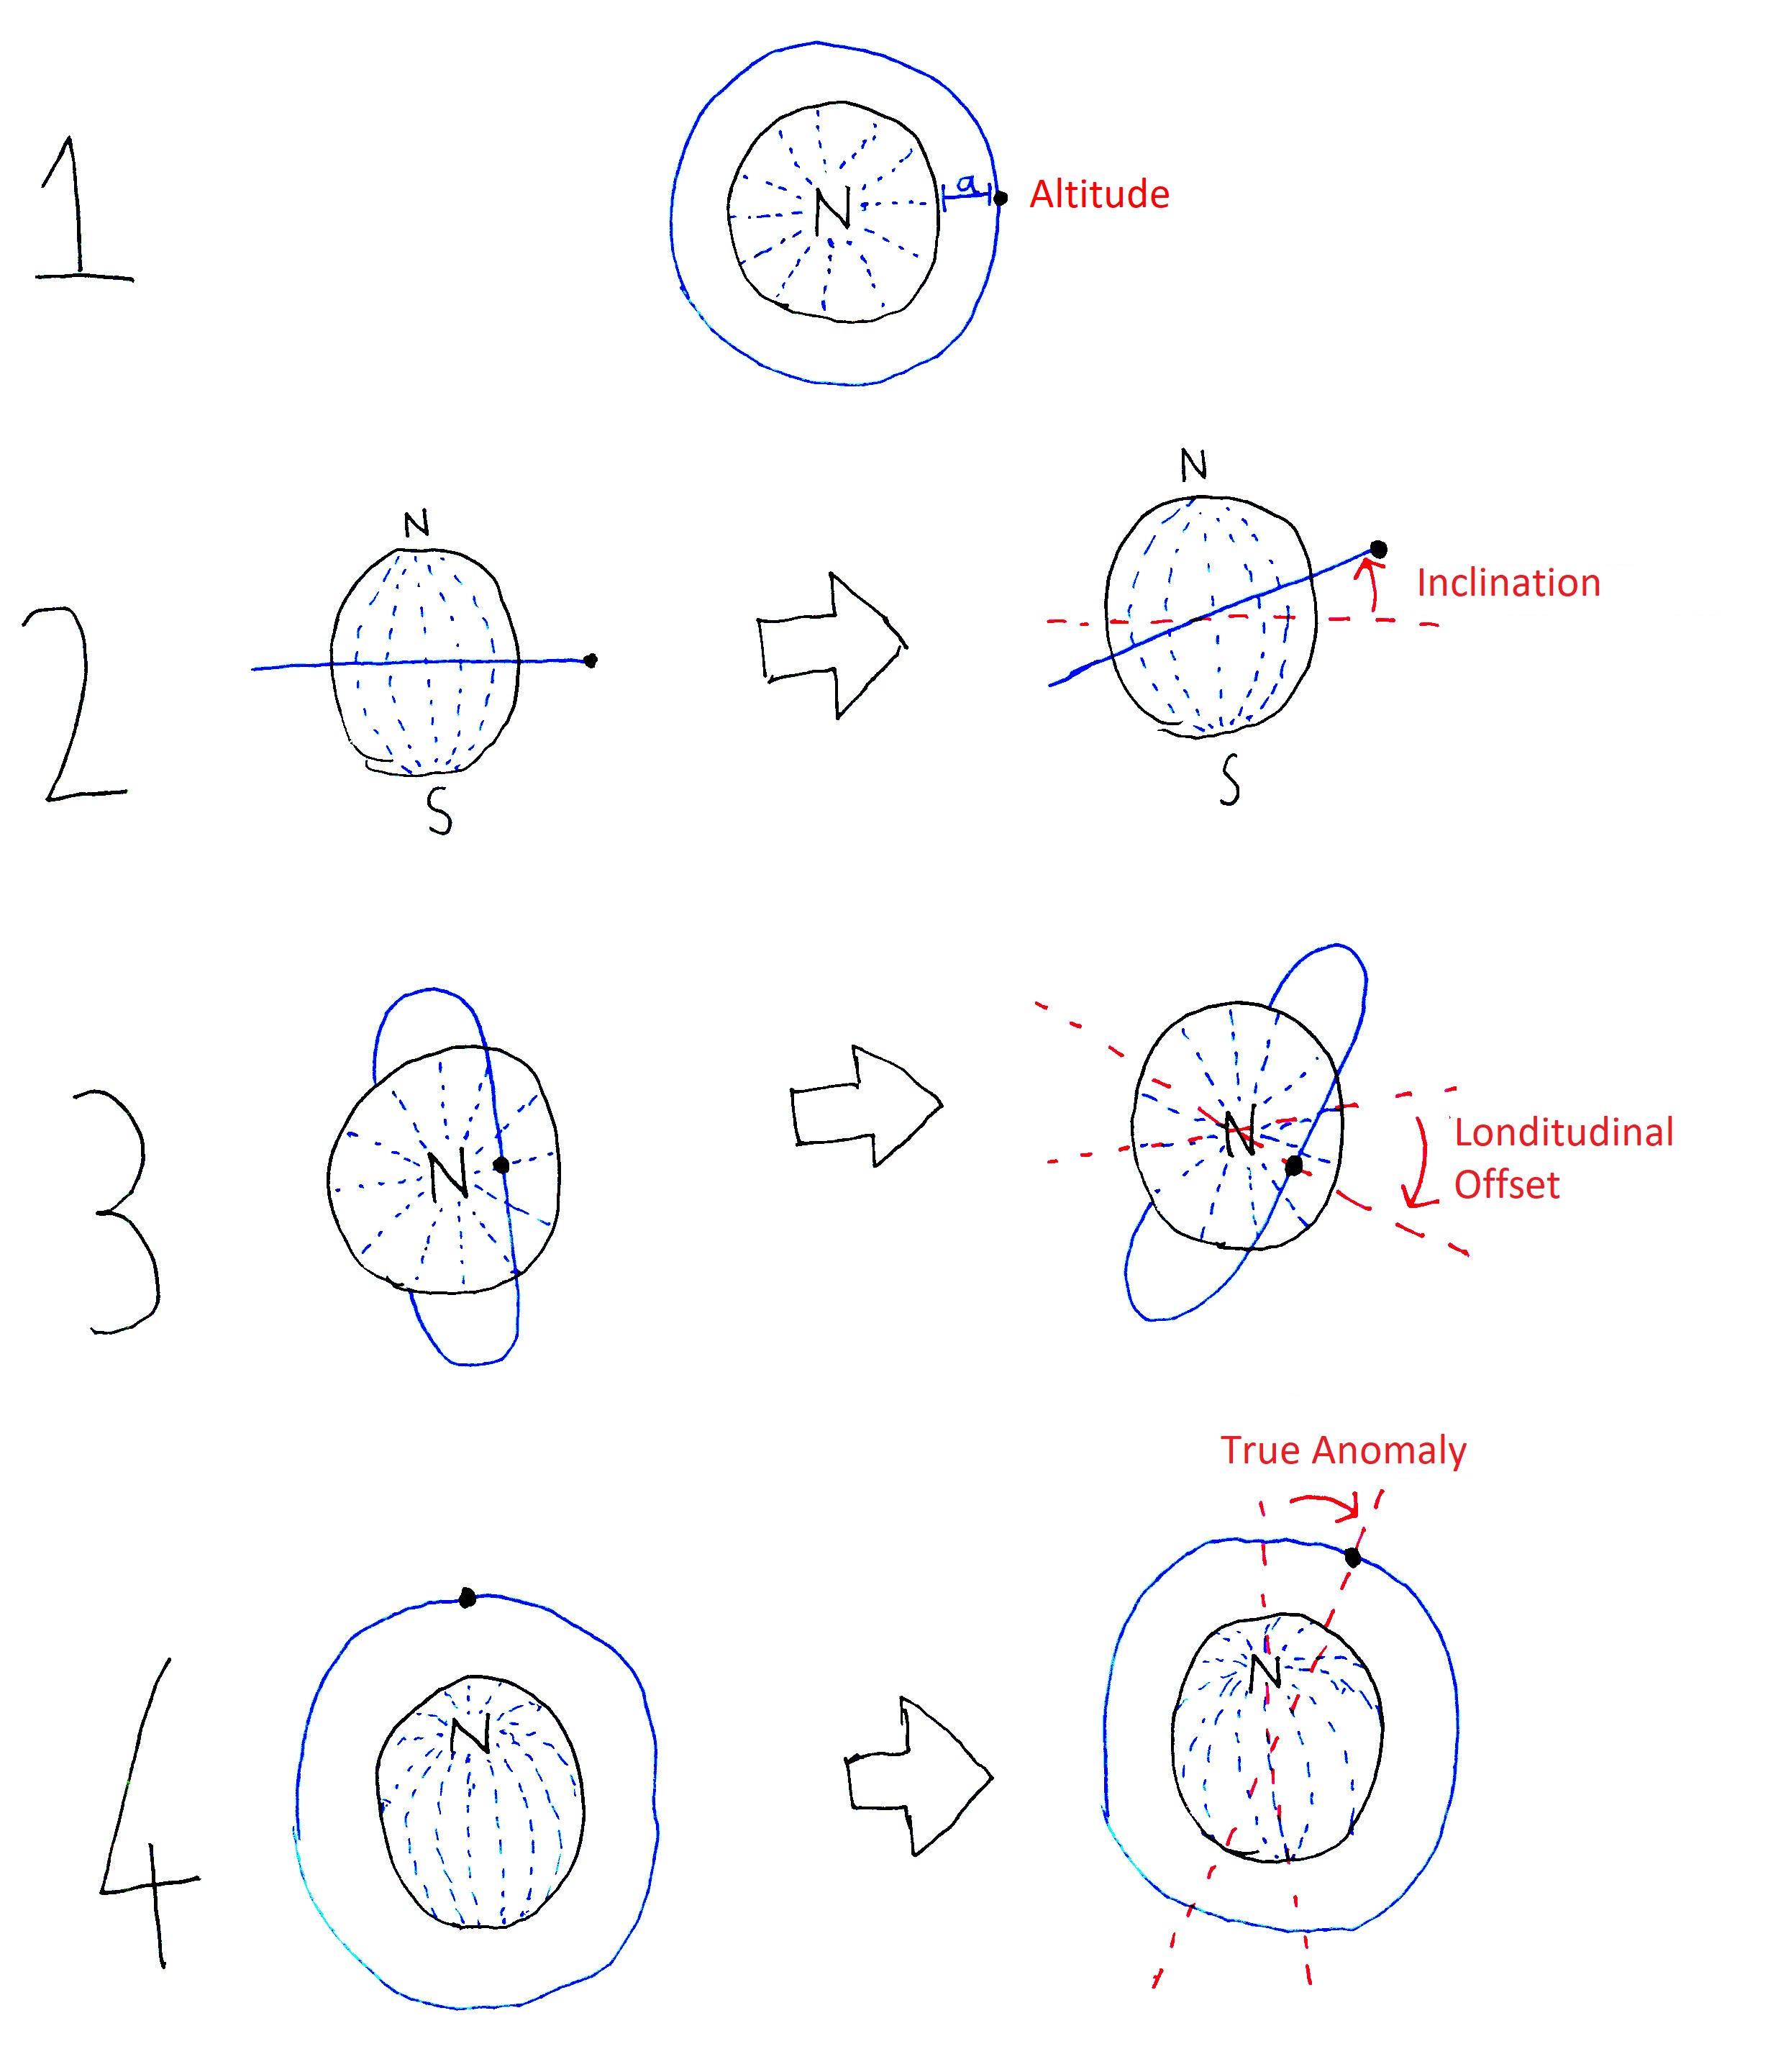
\includegraphics[width=\textwidth]{DescribingAnOrbit}
\end{figure}

Note that the altitude, inclination, and longitudinal offset together describe a circular orbit, with the true anomaly then specifying a location on this orbit to place our satellite.

Also not that this only describes circular orbits. There is another factor called eccentricity that describes how "squashed" the orbit is in shape. For the purposeless of this model we will assume eccentricity to be 0, as SpaceX have not applied for a high-eccentricity orbit\cite{FCCApplication}, and 0 eccentricity orbits are significantly easier to model (see below).


While these 4 values can describe the position of a satellite in space and it's orbit, they do not describe how the satellite moves. For this we need two more variables.

\begin{description}
\item[Initial Anomaly]
This is the satellite's true anomaly at time 0.
\item[Retrograde Status]
A Boolean variable. A retrograde orbit is one that goes against the rotation of the earth, typically these are described by orbits with a longitudinal offset greater than 180\degree. It is significantly more expensive to put a satellite into a retrograde orbit, and is essentially never done.\cite{Book}
\end{description}

Together, the Altitude, Inclination, Longitudinal Offset, Initial Anomaly and Retrograde Status uniquely determine a function that takes a time, and returns the position in 3D space that our satellite will be occupying at that time. It does this by first calculating the true anomaly, and then applying the transformations detailed in figure \ref{Describing an orbit} to translate this into a location. The rate of change of true anomaly, the angular velocity, is given by:

\[\sqrt{\frac{GM}{r^3}}\]

Where r is the distance from the origin, or altitude + radius of the Earth.

Note that while altitude is constant (eccentricity = 0) velocity is unchanging, and true anomaly can be described as a linear function of time.

\[TrueAnomaly(t) = InitialAnomaly + t * sqrt{\frac{GM}{r^3}}\]

Or $TrueAnomaly(t) = InitialAnomaly - sqrt{\frac{GM}{r^3}}$ if the orbit is retrograde.

Because the formula for calculating the position of a satellite at a given time is so easy to compute, we can calculate these values in advance, and then linearly interpolate between a series of fixed points to approximate the satellite motion. This means we do not run the same risks normal discrete physics models face when describing continuous behavior, such as the energy of the system changing, or orbital precession (the point of furthest distance moving steadily), as we will not be approximating a continuous process from a series of discrete steps but instead will be taking samples from a continuous function.

For the rest of this document, a satellite will be denoted by $x_{i,j,k}$. Describing the kth satellite on the jth orbital place in the ith orbital sphere. $L$ gives the number of orbital spheres, with $M_i$ giving the number of orbits in orbital sphere i, and $N_i,j$ giving the number of satellites in the jith orbit of the ith sphere. The jth orbit in the ith sphere will be denoted $o_{i,j}$, and the ith sphere will be denoted $s_i$

%===================================================UNKOWN VARIABLES========================================================
\section{Unknown Variables}
While we can learn a lot from SpaceX's applications, there are still a number of variables that are left undetermined. 

\begin{description}	
\item[Phase Offset]
As we do not know for certain how satellites will be positioned in orbits, we also do not know how they will be positioned relative to other orbits.
\item[Sphere Offset]
As well as satellites being offset from one another, whole spheres can be offset too. I will only be looking at a single sphere in my study, however, so this variable will not be examined.
\item[Link usage]
Each satellite will have a maximum of 4 links, however, we do not as of yet know which arrangements of links are the most optimal.
\end{description}

In my implementation I will go through how I described linking methods. 

%===================================================PHASE OFFSET========================================================
\section{Phase Offset}
In Mark Handley's paper he went through a method of describing phase offset that I will use in my implementation, outlined in figure \ref{Phase Offset}. Here we are looking at three adjacent orbits with a phase offset of 0, and then with a phase offset of a/b, the empty red circles give where a satellite would have been if the phase offset was 0. As you can see the phase offset is a value between 0 and 1 that describes the displacement of satellites in each orbit relative to one another. With 0 meaning that satellite $x_{0,0,0}$ crosses the equator at the same time as $x_{0,1,0}$, 1 meaning that $x_{0,0,0}$ crosses at the same time as $x_{0,1,1}$, and other values being a linear interpolation between these two states.

\begin{figure}
	\caption{Phase Offset described by looking at three adjacent orbits.}
	\label{Phase Offset}
	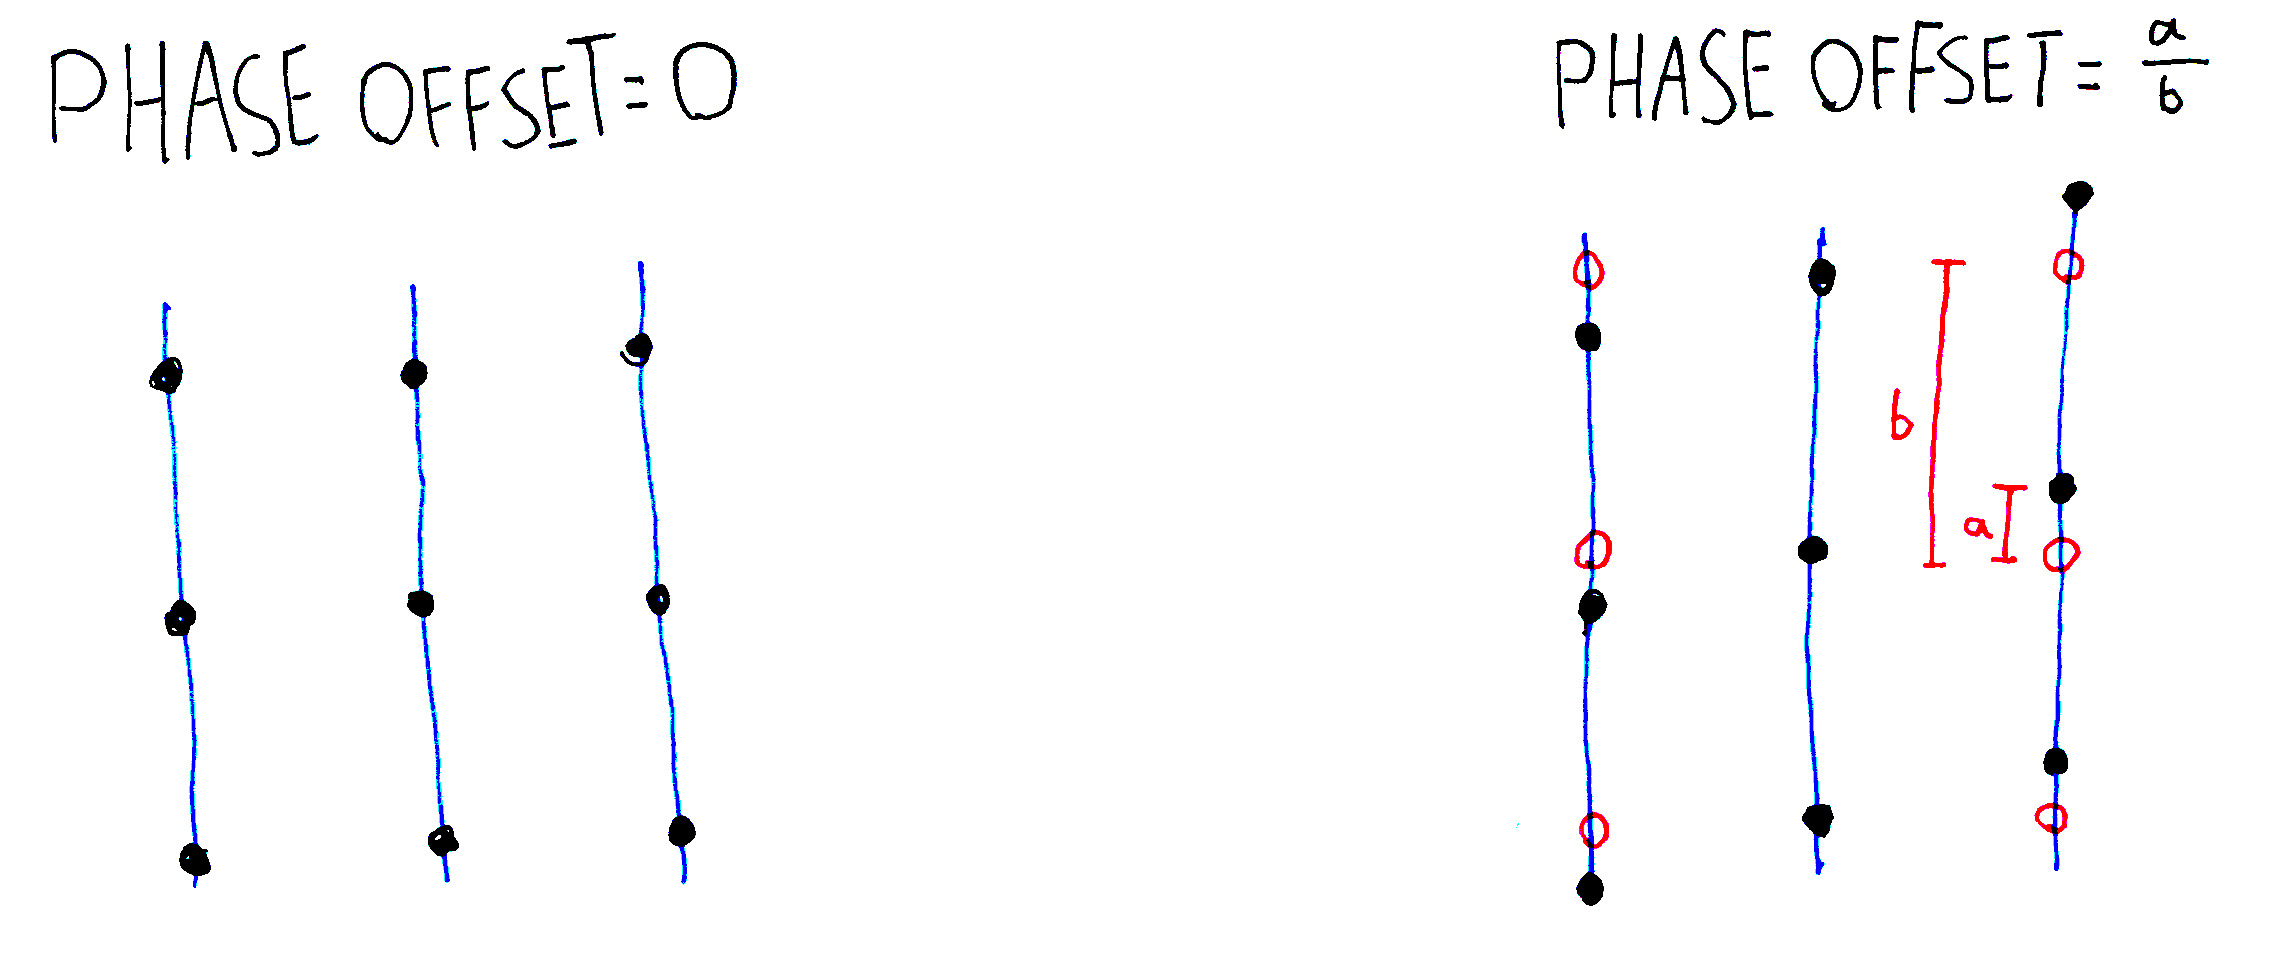
\includegraphics[width=\textwidth]{PhaseOffset}
\end{figure}

Because the constellation wraps around the earth, with $o_{i,M_i} = o_{i,0}$, it is necessary that the phase offset be a multiple of $1/N_i,0$, so that the accumulated phase offset at $o_{i,M_i}$ results in an arrangements of satellites identical to $o_{i,0}$. In Mark Handley's research, he the optimum for the Starlink network to be 9/33. Which I will use in my research.

%===================================================STARLINK========================================================

All the details that we know about the Starlink constellation going into implementation are given in figure \ref{fig:Starlink Within Program}. What will need to be determined upon implementation is how to describe the linking method.

\begin{figure}
\caption{An example for how a constellation might be described.}
\label{fig:Starlink Within Program}
\begin{center}
\begin{tabular}{ | c | c  | }
	\hline
	Number of Orbital Spheres & 1 \\
	Altuitude & 550km \\
	Inlication & 53\degree\\
	Number of Orbits & 24\\
	Sattellites per Orbit & 66\\
	Phase Offset & 9/66\\
	\hline
\end{tabular}
\end{center}
\end{figure}

%==============================================================================================================================
%----------------------------------------------------------------------------------------------------------IMPLEMENTATION----------------------------------------------------------------------------------------------------
%==============================================================================================================================
\chapter{Implementation}

%============================================REPOSITORY OVERVIEW======================================================
\section{Repository Overview}

%============================================CODING FOR VISUALISATION AND EFFICENT ALGORITHMS======================================================
\section{Coding for Visualisation and Efficent Algorithms}

This implementation chapter is divided into two main sections, the first section will go over how I represented the constellations and the code I wrote to perform tests on this model, the second section will go over the executable file, it's structure, and how to use it. While these sections are separate in my report, they were developed concurrently, and are connected to each other.  As I visualized the constellation, I was able to gain a better understanding of it's structure, this directed the properties of the network I wanted to examine, which in turn effected the tests I wanted to create and so the algorithms I needed to implement. Furthermore as Godot is designed to model 3D environments it provides a number of functions that in turn influenced how I wrote my algorithms, most notably Godot provides a simple framework for multi-threading through a \lstinline{_process} function that any class extending Node can override and which is called on every step by the engine. Godot handles multi-threading of the \lstinline{_process} function internally. This gave me the opportunity to exploit threading to improve the efficiency of the program without having to do any extra work. All that said, I think to is clearer to divide these two halves of the program when talking about my implementation.

After these two sections will be one more outlining observations that were made of the network's behavior during my experimenting on it, and how these observations lead to further development in my linking algorithms.

%============================================MODELING THE NETWORK======================================================
\section{Modeling the Network}

%-----------------------------------------------------------------------------PATTERNS USED-----------------------------------------------------------------------------
\subsection{Patterns used}

Due to the extensive combustibility of the network, I elected to use the Template Method pattern in three separate locations.

\begin{itemize}
\item To describe different linking methods.
\item To describe various different ways of colorizing the network to highlight certain properties.
\item To describe various tests to be applied to the network.
\end{itemize}

I also utilized a variant of the Builder pattern for describing constellations and tests. The ConstellationDescription class is initialized with a description of a constellation similar to what was given above, including the tests and coloring method I want to use on the class. This allowed me to easily categorize and load new constellations.


%-----------------------------------------------------------------------------MODELLING SATELLITE POSITIONS-----------------------------------------------------------------------------
\subsection{Modeling Satellite Positions}
I initially did not precompute orbits but instead had every satellite recalculate it's position on every step. On Implementation, I found that this was flawed, being able to simulate only 500 satellites in motion before slowing down. Because of this, I changed to a precomputed method. In this method, orbits are precomputed as a number of transformations, and the position of satellites is calculated by interpolating adjacent transformations, this sacrifices some accuracy, but vastly increases the computation speed. It is important that orbits be described by transformations (a combination of a point and rotation) so that satellites can be oriented to ways have the earth below them from their reference frame. This makes a number of computations later on easier.

There are five overall classes for representing the different objects that make up a constellation.

\begin{description}
\item[Constellation] This is an overall class that contains a list of BaseStations and a list of OrbitalSpheres. Each step the constellation will run any programs that cannot be threaded, this include parts of the Linking Method, calculating the current rotation of the Earth, and any test that is being presently ran on the network.
\item[BaseStation] Describes  surface level station. Each step it moves to match the rotation of Earth.
\item[OrbitalSphere] Each step this updates an internal value known as "RotationOfOrbit". As all orbits in the same orbital sphere are at the same altitude, all the satellites in these orbits have the same angular momentum, it is therefore possible to store the rotation of all of these orbits in the same place to ensure they remain in sync. OrbitalSphere contains a list of Orbits.
\item[Orbit] An orbit contains a list of Satellites. It is the Orbit objects that do most of the work in calculating the positions of Satellites. They store a list of satellites along with a precomputed list of points that describe their orbit, each step they look at the RotationOfOrbit of their parent class and update the positions of the satellites in their list accordingly. It also calculates some of the information used for the LinkingMethod each step.
\item[Satellite] The Satellite class is a simple descriptor that stores information related to the satellite. Satellite objects do not posses a \lstinline{_process} function that is called each step as this would be too costly for thousands of satellites to do.
\end{description}

Between them these classes can model the motion of an entire constellation with ground stations. Note however that they do not visualize it. To have something be visualized in Godot you have to add a "scene" containing a "node" to the "scene tree". Node can have associated scripts that they call the functions of, which is what these 5 classes are, but this it is worth bearing in mind that the "Satellite" class is not visualized, but rather instanced by a a node object called Satellite that is then visualized. I will go into how this works in the second section.

%-----------------------------------------------------------------------------REPRESENTING LINKS-----------------------------------------------------------------------------
\subsection{Representing Links}
There are 3 primary ways to represent a graph for algorithms:

\begin{description}
\item[Adjacency Matrix] An NxN matrix of values representing all possible connections. Obviously inefficient for a sparse set of connections like this.
\item[Adjacency List] Associate each Satellite with a list of the vertices it is connected to. Space efficient, but creates difficulty in running Dijkstra's algorithm.
\item[Edge List] Create a list of edges that refer to vertices. This is useful for algorithms that require iterating through all edges like Dijkstra's algorithm. But to find the adjacent satellites to any given satellite requires searching through the whole list.
\end{description}

Initially, I used adjacency lists, this lead to a number of problems.

\begin{itemize}
\item Some algorithms require a list of all edges, which is very hard to obtain with adjacency lists.
\item When drawing edges in the visualization, each would be drawn twice, for each vertex they were associated with.
\item When updating links, values such as the distance between two vertices had to be computed twice for each vertex.
\end{itemize}

Instead I created a new class of objects representing links, and gave each vertex a reference to the links associated with it. 

In Godot, all drawn objects require one "parent" (different to class inheritance) which is already a drawn object. Children inherit the position and rotation of their parents, and rotating a group of objects is significantly more efficient than rotating a single object alone. Because of this, backwards and forward links, which do not change distance or position relative to the satellite, should be made children of the satellite, and they will then never have to be updated. Because of this, all links have a primary and secondary satellite. Which the link always being the child of the primary satellite.

%-----------------------------------------------------------------------------REPRESENTING LINKING METHODS-----------------------------------------------------------------------------
\subsection{Representing Linking Methods}
As well as having a way to describe a link between two satellites I needed a way to describe the linking method used to form these links. To do this I used the Template Method pattern outlined above, however after experimenting with numerous different linking methods, I ended up settling on just two.

\begin{description}
\item[NoLinking]
\item[FixedLinking(X)]
\end{description}

Fixed Linking is created with a matrix that can be customized to describe a huge range of potential linking methods. I will describe how this works below.

Fixed linking describes a linking method where links are constant, and each satellite links to it's neighbors in the same way, this creates a network with a grid-like topology. As links are bidirectional and all satellites have fixed, identical linking patterns, satellites must have an even number of links available to them, as the number of satellites they are "linking to" will be identical to the number that are "linking to them".

Fixed linking is initialized with a nx2 matrix, where n is half the number of links per satellite, and columns of the matrix correspond to the satellites that are linked to. Like so:

\[\begin{bmatrix} 
Positions Forward in Orbit 1 & Positions Forward in Orbit 2 \\
Positions to the Left 1 & Positions to the Left 2\end{bmatrix}\]

So:

\[FixedLinking(\begin{bmatrix} 
1 & 0 & 1 \\
0 & 1 & 1\end{bmatrix}\]

Describes a linking method where each satellite has 6 links available, and connects to the satellite directly in front ($\begin{bmatrix}1\\0\end{bmatrix}$), to the left ($\begin{bmatrix}0\\1\end{bmatrix}$), and diagonally forward and to the left ($\begin{bmatrix}1\\1\end{bmatrix}$), as well as forming connections with the three satellites it is in front of, to the left of, and forward-left of.

However, there is a difficultly here when it comes to phase offset. Because of the way phase offset accumulates between orbits, $x_{0,M_0-1,0}$ is not necessarily to the right of $x_{0,0,0}$. Because of this an adjustment must be made between $o_{i,M_i}$ and $o_{i,o}$ to correct, as outlined in figure \ref{Linking Method and Phase Offset}. Also i this figure I have given an example of a linking method with negative value.

I decided to dub linking methods of the form:

\[FixedLinking(\begin{bmatrix} 
1 & x \\
0 & 1\end{bmatrix}\]

As "Handley(x)" or "H(x)" linking methods, as they are the forms of linking that Mark Handley examined in his original paper.

\begin{figure}
	\caption{The relationship between the linking method used and phase offset.}
	\label{Linking Method and Phase Offset}
	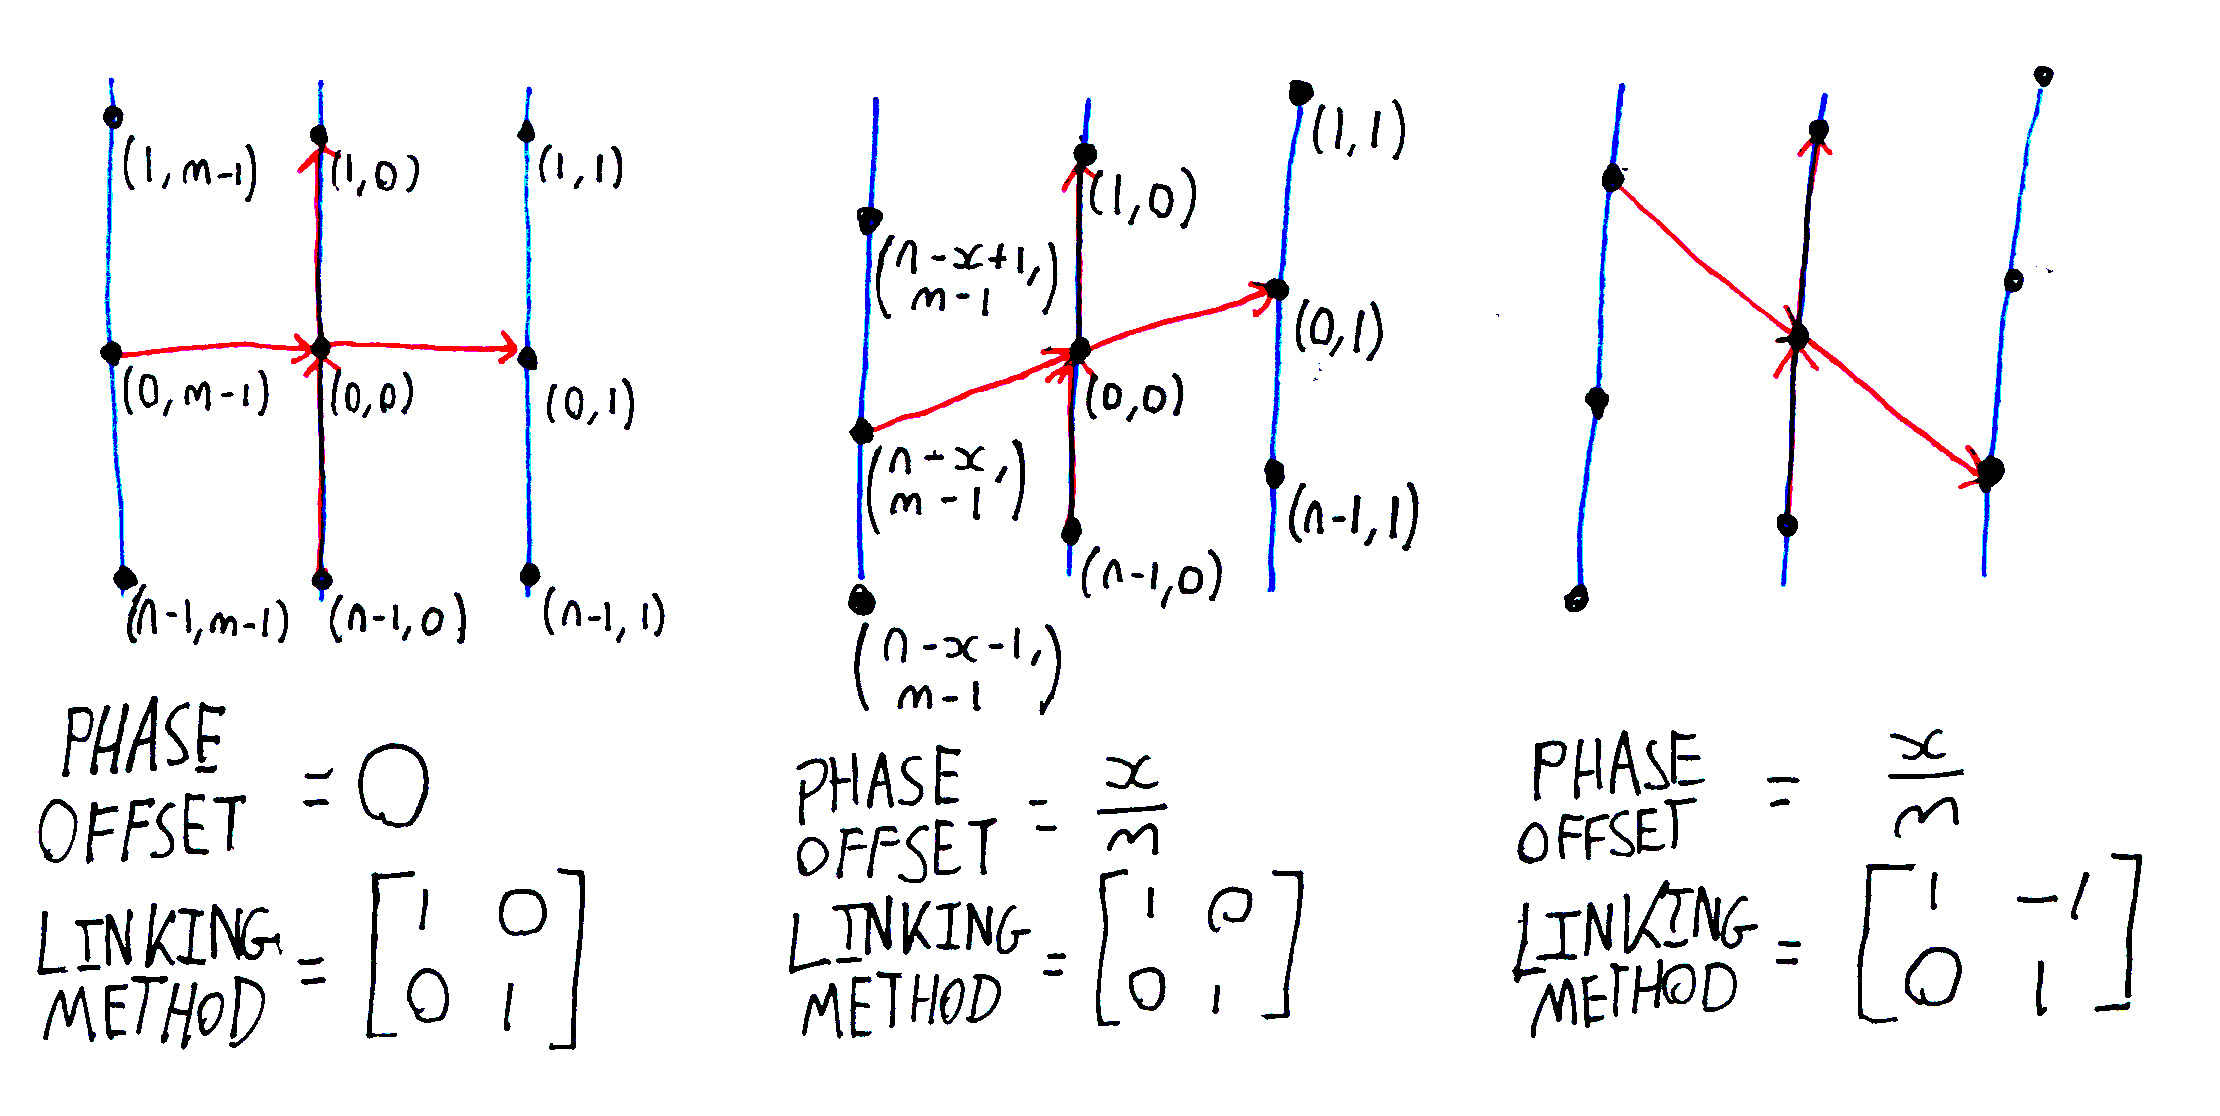
\includegraphics[width=\textwidth]{LinkingMethodAndPhaseOffset}
\end{figure}

%-----------------------------------------------------------------------------REPRESENTING TESTS-----------------------------------------------------------------------------
\subsection{Representing Tests}
Tests were associated with a constellation and ran every step. However, to prevent slowing down, when a test ran it would check the system clock, and each second would run it's main code and produce outputs. Using the system clock might have posed a problem as in game time and system time might go our of sync, but Godot has inbuilt functionality to ensure that processes are kept in sync with system time, objects that are called with the \lstinline{_process} function are passed a float that represents the amount of system time that has passed since the last \lstinline{_process} call, by using this value in all my physics simulations I was able to guarantee that my program stayed in sync with system time.

All the tests had an associated file that they would output their results into, as well as logging them on the terminal, in csv format. Not all the computations were done by my code however, and some of the csv files had to be processed in spreadsheets to produce meaningful data.

%-----------------------------------------------------------------------------CONECTED COMPONENETS-----------------------------------------------------------------------------
\subsection{Connected Components}
One of my tests required me to calculate the number of connected components. This was done very simply through a number of depth-first searches starting at unvisited nodes until all nodes had been visited.

%-----------------------------------------------------------------------------DIJKSTRA'S ALGORITHM-----------------------------------------------------------------------------
\subsection{Dijkstra's Algorithm}

I used Dijkstra's algorithm in order to calculate shortest paths around the network, with the modification to allow for quickly retrieving the shortest path when used. Somewhat surprisingly, C sharp doesn't come with a priority queue, so I used one sourced from 2 different tutorials. Taking the structure of one and then implementing the quick comparison operations from another.\cite{PriorityQueue1}\cite{PriorityQueue2}

%-----------------------------------------------------------------------------CALCULATING LATENCY ACROSS PATH-----------------------------------------------------------------------------
\subsection{Calculating the Latency Across a Path}

There are 4 factors that effect the latency of a path, some of which are easy to model, and others are significantly more tricky.

\begin{description}
\item[Processing delay] The time it takes router to process the packet header, this is typically insignificant and will bee assumed to be 0.
\item[Queuing delay]  The time the packet spends in routing queues, this is dependent on the load on the network and is therefore not easy to predict. I will be calculating latency assuming the best case scenario, which is no queuing delay.
\item[Transmission delay] The time it takes to push the packet onto the link. This is of course dependent on the size of the packet, but for the smallest packet sizes this value is negligible. 
\item[Propagation delay] The time the signal spends in transmission, since all connections are of the form of electromagnetic waves this is simply the path length divided by the speed of light.
\end{description}

Because of this, the only calculation needed to calculate needed to get the latency of a path is to divide it's length by the speed of light in a vacuum. To calculate the round trip time (RTT), which is typically used when advertising linking systems, we simply multiply this value by two.

%-----------------------------------------------------------------------------EFFICIENCY VS USABILITY-----------------------------------------------------------------------------
\subsection{Efficiency vs Usability}
My code went through about 2 major rewrites, and over the course of this I ended up using numerous abstract classes and wrappers that would simplify more complex objects. There are two kinds of vertex, base stations and satellites, and two kinds of link, those between satellites and those between a satellite and base station. Each of these are children of general Vertex and Link classes, and it is these classes that are used by the various tests and algorithms that run on the network. Initially my objective was to prioritize efficiency at all costs, but as I continued to develop the code, it became necessary to implement redundancies and inefficient storing methods, like lists, in order to make the code more easily usable. I also created a generic Graph object that contained only a list of Vertices and a list of Links, and a VertexParth object that allowed for easy manipulation and testing of paths.

%============================================VISUALISATION======================================================
\section{Visualization}


%-----------------------------------------------------------------------------HOW TO USE THE EXE------------------------------------------------------------------------------------

\subsection{How to Use the EXE}

If you would like to see the program that was used to generate these images and results, simply download and run the exe stored with the code.

The exe will create files for test results in the same location as it is ran, as well as printing to the command line the results of tests as they are written.

It is recommended that you run in Windows 10, as it is not guaranteed to work in other operating systems.

You can navigate the simulation using the mouse, along with arrow keys or WASD. Press R to reset the whole simulation. Use X and Z to move between different tests. Press ESC to toggle the mouse between captured (for moving the camera) and free.

All the tests run at 60x realtime, which I found to be a very good timefactor for observing overarching trends in the network.

\begin{figure}
\begin{center}
\label{fig:Keybindings}
\caption{Keybindings.}
\begin{tabular}{ | c | c  | }
	\hline
	Move Forward & W, Up Arrow \\
	Move Backward & S, Down Arrow\\
	Move Up & Q, Comma Key\\
	Move Down & E, Full Stop Key\\
	Move Left & A, Left Arrow \\
	Move Right & D, Right Arrow \\
	Restart Simualtion & R \\
	Toggle Free Mouse & Esc \\
	Next Scene & X\\
	Previous Scene & Z\\
	\hline
\end{tabular}
\end{center}
\end{figure}

There are a total of 17 scenes available. I will list them here, though at this point in the report it might not be clear what they mean.

\begin{enumerate}
\item Gradient Applied to Each Orbit
\item Following a Satellite and it's Neighbors
\item Handley(-1)
\item Handley(0)
\item DistantLinking
\item Connected Components with Deletetions: Handley(-1)
\item Connected Components with Deletetions: Handley(0)
\item Connected Components with Deletetions: DistantLinking
\item Shortest Path London-New York with Deletions: Handley(-1)
\item Shortest Path London-New York with Deletions: Handley(0)
\item Shortest Path London-New York with Deletions: DistantLinking
\item Shortest Path Beijing-New York with Deletions: Handley(-1)
\item Shortest Path Beijing-New York with Deletions: Handley(0)
\item Shortest Path Beijing-New York with Deletions: DistantLinking
\item Shortest Path London-Johannesburg with Deletions: Handley(-1)
\item Shortest Path London-Johannesburg with Deletions: Handley(0)
\item Shortest Path London-Johannesburg with Deletions: DistantLinking
\end{enumerate}

Tests 6 to 17 will all run by themselves, moving over to the next scene once they are complete and outputting their results into a folder called TestResults. However it will take over 24 hours in total to run all of these tests and output their results.

%-----------------------------------------------------------------------------THE MOTION OF THE PLAYER------------------------------------------------------------------------------------
\subsection{The Motion of the Player}

One of the few pieces of code written in Godot's native language GDScript is the code that controls user interaction with software. It made sense to write this in GDScript as it is a much simpler language than C\#, and because a very simple tutorial of first person motion was available in GDScript\cite{FirstPersonMotion}. However this code required some adaptation to make it work for my purposes, primarily the removal of a number of unnecessary features, and the addition of the ability to move up and down.

The code works using a "head" which is attached to a "neck". Left-right motions of the mouse are translated to left-right rotations of the neck, while up-down motions of the mouse are translated into up-down rotations of the head. keeping the head and neck separate mean that the player cannot turn themselves upside down. Motion is done relative to the head's view, with gentle smoothing applied to motion to give a more natural feeling.

%-----------------------------------------------------------------------------AESTHETIC IMPROVEMENTS------------------------------------------------------------------------------------
\subsection{Aesthetic Improvements}
I made a number of adjustments to the code in order to make images look clear in my report. I chose a while background opposed to the black of space, and used a low-saturation, simplified image of Earth instead of a more realistic image so that links would show up more clearly over it. For the Earth texture I used a creative commons equirectangular map of the Earth. Equirectangular means that x and y values correspond to longitude and latitude. It was important that the map be equirectangular as this is the format that is compatible with being mapped to a sphere. \cite{Map} I also added a soft light source, as this is extremely easy to do in Godot and goes a long way to making the cubes of the satellites appear more clearly and the overall image more pleasant.

I developed a number of different Coloring Methods using the method pattern that allowed me to customize the colors of the various objects in the scene. This was extremely useful as different tests require different ways of highlighting the network to make it clear what I am trying to visualize.

%============================================INITIAL OBSERVATIONS OF THE NETWORK======================================================
\section{Initial Observations of the Network}

While working on the program I made a few notable observations of the network. In this section I go through each of these observations and outline how it fed into what I was doing.

%-----------------------------------------------------------------------------THE STRUCTURE OF THE NETWORK------------------------------------------------------------------------------------
\subsection{The Structure of the Network}

One of the most notable observations of the network was it's unique, layered grid structure. To highlight this I applied a different hue to each orbit \ref{fig:Structure of Network}. As you can see, for a given point near the equator, there are in fact two very different kinds of Satellite moving overhead, those going North-East, and those going South-East. Towards the poles, on the other hand, all satellites are moving Eastward. This means that Satellites that pass very close to one another on the equator can end up on opposite sides of the Earth close to the poles. As described below, it is very likely that Satellites will only link to other satellites moving the same direction as them, and in my model I have reflected that. This means that for a given point on earth there will be two almost separate grids moving overhead, one grid of satellites moving North-East, and another of satellites moving South-East.

\begin{figure}
\label{fig:Structure of Network}
\caption{The Starlink Constellation with a different hue applied to each orbit.}
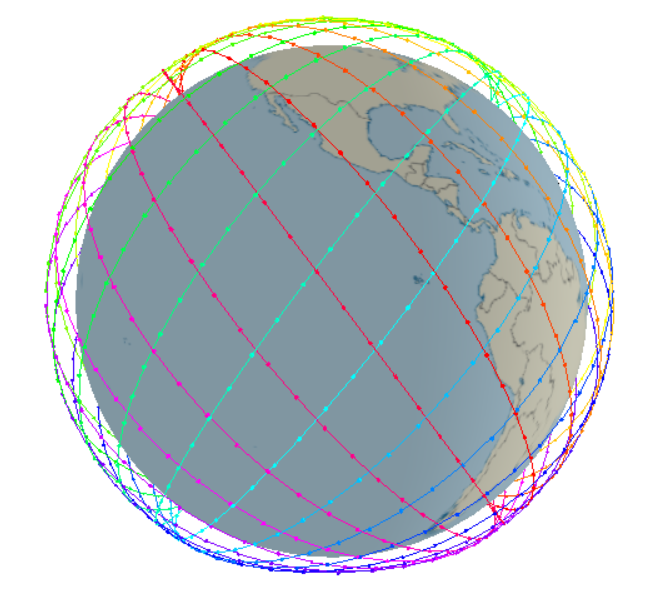
\includegraphics[width=0.3\textwidth]{Hue1}
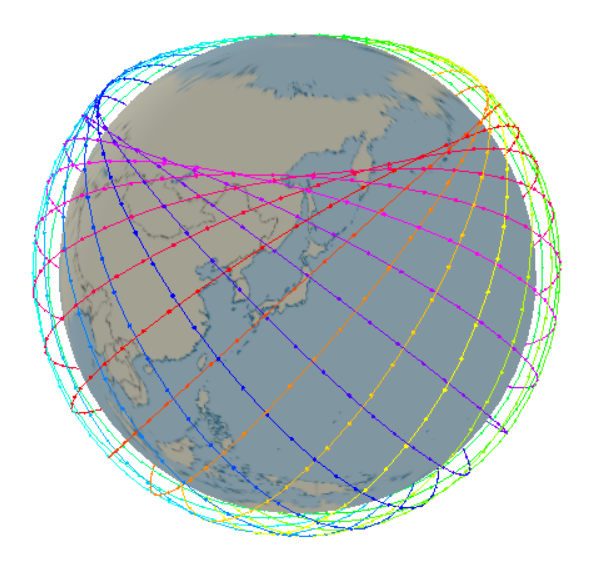
\includegraphics[width=0.3\textwidth]{Hue2}
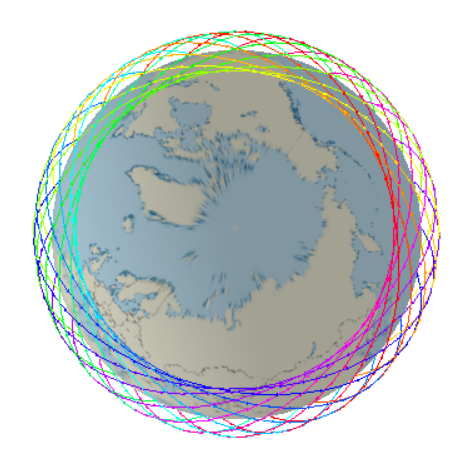
\includegraphics[width=0.3\textwidth]{Hue3}
\end{figure}

%-----------------------------------------------------------------------------THE MOVEMENT OF SATELLITES RELATIVE TO EACH OTHER------------------------------------------------------------------------------------
\subsection{Movement of Satellites Relative to Each Other}

I decided to track the path of a satellites neighbors relative to it and it's direction of movement over the course of an orbit around the Earth. In figure  \ref{fig:Relative Paths of Satellites} the paths traced by nearby satellites is given. The satellites directly ahead of and behind a given satellite stay in a steady position relative to it and it's direction of motion, while those in adjacent orbits slowly figure eights. You can see in figure \ref{fig:The 9 Satellites Being Tracked} that there are other nearby satellites in different orbits, however these satellites are moving South while the highlighted satellites are moving North, meaning that they will be moving by far too quickly for the main satellite to track them as they pass. \cite{OriginalReport}

These results show that satellites in adjacent orbits will be moving in relatively slow and predictable ways meaning it should be possible for a satellite to track a laser link to satellites in adjacent orbits. It also shows that links to satellites in the same orbit will be significantly easier as satellites in the same orbit maintain a constant position relative to one another.

\begin{SCfigure}
\centering
\caption{The 9 Satellites I tracked, the motion was logged relative to the position and direction of motion of the central satellite.}
\label{fig:The 9 Satellites Being Tracked}
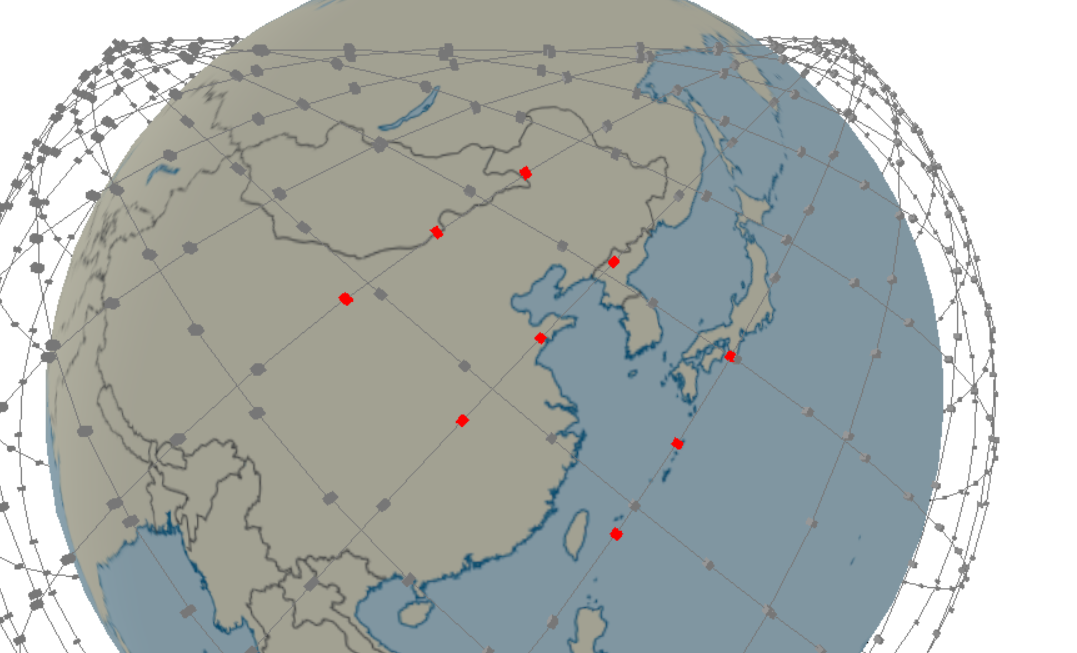
\includegraphics[width=0.5\textwidth]{NearbySats}
\end{SCfigure}

\begin{figure}
\centering
\caption{An example of the paths that neighbors take relative to a satellite and it's direction of motion.}
\label{fig:Relative Paths of Satellites}
\begin{tikzpicture}
\begin{axis}  [xlabel={Distance Perpendicular to Direction Of Motion (km)}, ylabel={Distance in Direction of Motion (km)},width=\textwidth]
\addplot [mark=*, color=black] table [x expr = \thisrow{sat0x} * 1000, y expr = \thisrow{sat0z} * 1000, col sep=comma] {./Data/NearbySats.csv};
\addplot [mark=*, color=red] table [x expr = \thisrow{sat1x} * 1000, y expr = \thisrow{sat1z} * 1000, col sep=comma] {./Data/NearbySats.csv};
\addplot [mark=*, color=orange] table [x expr = \thisrow{sat2x} * 1000, y expr = \thisrow{sat2z} * 1000, col sep=comma] {./Data/NearbySats.csv};
\addplot [mark=*, color=yellow] table [x expr = \thisrow{sat3x} * 1000, y expr = \thisrow{sat3z} * 1000, col sep=comma] {./Data/NearbySats.csv};
\addplot [mark=*, color=green] table [x expr = \thisrow{sat4x} * 1000, y expr = \thisrow{sat4z} * 1000, col sep=comma] {./Data/NearbySats.csv};
\addplot [mark=*, color=blue] table [x expr = \thisrow{sat5x} * 1000, y expr = \thisrow{sat5z} * 1000, col sep=comma] {./Data/NearbySats.csv};
\addplot [mark=*, color=purple] table [x expr = \thisrow{sat6x} * 1000, y expr = \thisrow{sat6z} * 1000, col sep=comma] {./Data/NearbySats.csv};
\addplot [mark=*, color=gray] table [x expr = \thisrow{sat7x} * 1000, y expr = \thisrow{sat7z} * 1000, col sep=comma] {./Data/NearbySats.csv};
\end{axis}
\end{tikzpicture}
\end{figure}

\begin{SCfigure}
\centering
\caption{Towards the South Pole, the square of satellites fold over and the satellites that were once on the right of the central satellite move to the left.}
\label{fig:Exchange of Satellites}
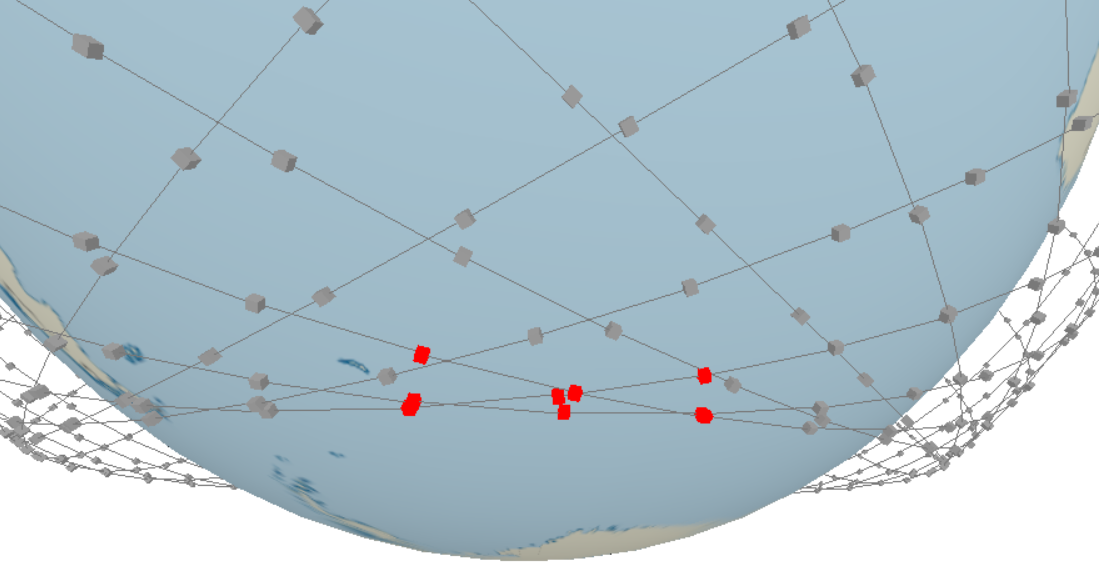
\includegraphics[width=0.5\textwidth]{NearbySats2}
\end{SCfigure}

\begin{figure}
\centering
\caption{The distance over time from a satellite to it's neighbors perpendicular to it's direction of motion and the direction towards the core of the Earth, or how far to the left or right of the satellite it's neightbors are over time.}
\label{fig:Sideways Position of Satellites}
\begin{tikzpicture}
\begin{axis}  [xlabel={Time Passed (minutes)}, ylabel={Distance Perpendicular to Direction of Motion (km)},width=\textwidth]
\addplot [mark=, color=black] table [x=time, y expr = \thisrow{sat0x} * 1000, col sep=comma] {./Data/NearbySats.csv};
\addplot [mark=, color=red] table [x=time, y expr = \thisrow{sat1x} * 1000, col sep=comma] {./Data/NearbySats.csv};
\addplot [mark=, color=orange] table [x=time, y expr = \thisrow{sat2x} * 1000, col sep=comma] {./Data/NearbySats.csv};
\addplot [mark=, color=yellow] table [x=time, y expr = \thisrow{sat3x} * 1000, col sep=comma] {./Data/NearbySats.csv};
\addplot [mark=, color=green] table [x=time, y expr = \thisrow{sat4x} * 1000, col sep=comma] {./Data/NearbySats.csv};
\addplot [mark=, color=blue] table [x=time, y expr = \thisrow{sat5x} * 1000, col sep=comma] {./Data/NearbySats.csv};
\addplot [mark=, color=purple] table [x=time, y expr = \thisrow{sat6x} * 1000, col sep=comma] {./Data/NearbySats.csv};
\addplot [mark=, color=gray] table [x=time, y expr = \thisrow{sat7x} * 1000, col sep=comma] {./Data/NearbySats.csv};
\end{axis}
\end{tikzpicture}
\end{figure}

%-----------------------------------------------------------------------------INITIAL OBSERVATIONS OF LATENCIES LATENCIES------------------------------------------------------------------------------------
\subsection{Initial Observations of Latencies}

In figure \ref{fig:Latency London To New York} you can see an example of the kind of latencies that you might expect between two locations through the SpaceX network. As you can see the latency changes relatively slowly for periods, followed by sudden jumps. The sudden jumps represent when the a new path becomes available or an old path is broken, and a changeover happens, while the path is constant, the latency changes due to satellites moving away from or towards one another.

In figure \ref{fig:LDN-NY} you can see two different images of the shortest path between London and New York taking at different times. As you can see the shortest path between two locations can change somewhat dramatically over time, this accounts for the huge jumps that are seen in latency.

It's also worth noting that while these jumps are lengthy they are well below the maximum amount of jitter tolerated by VoIP protocols.\cite{HowMuchJitter}

\begin{figure}
\caption{The Latency of the London-New York connection over time}
\label{fig:Latency London To New York}
\begin{tikzpicture}
\begin{axis}  [width=\textwidth, height=\axisdefaultheight,  xlabel={Time (minutes)}, ylabel={RTT (milliseconds)}]
\addplot table [x expr=\thisrow{Time} / 60, y expr=\thisrow{Time of Signal (milliseconds)} * 2, col sep=comma] {./Data/LondonToNewYork.csv};
\end{axis}
\end{tikzpicture}
\end{figure}

\begin{figure}
	\centering
	\caption{Image of the shortest path between London and New York in Handley(-1) at two different times.}
	\label{fig:LDN-NY}
	\begin{subfigure}[b]{0.4\textwidth}
		\caption{The shortest path between London and New York, passing over the artic circle.}
		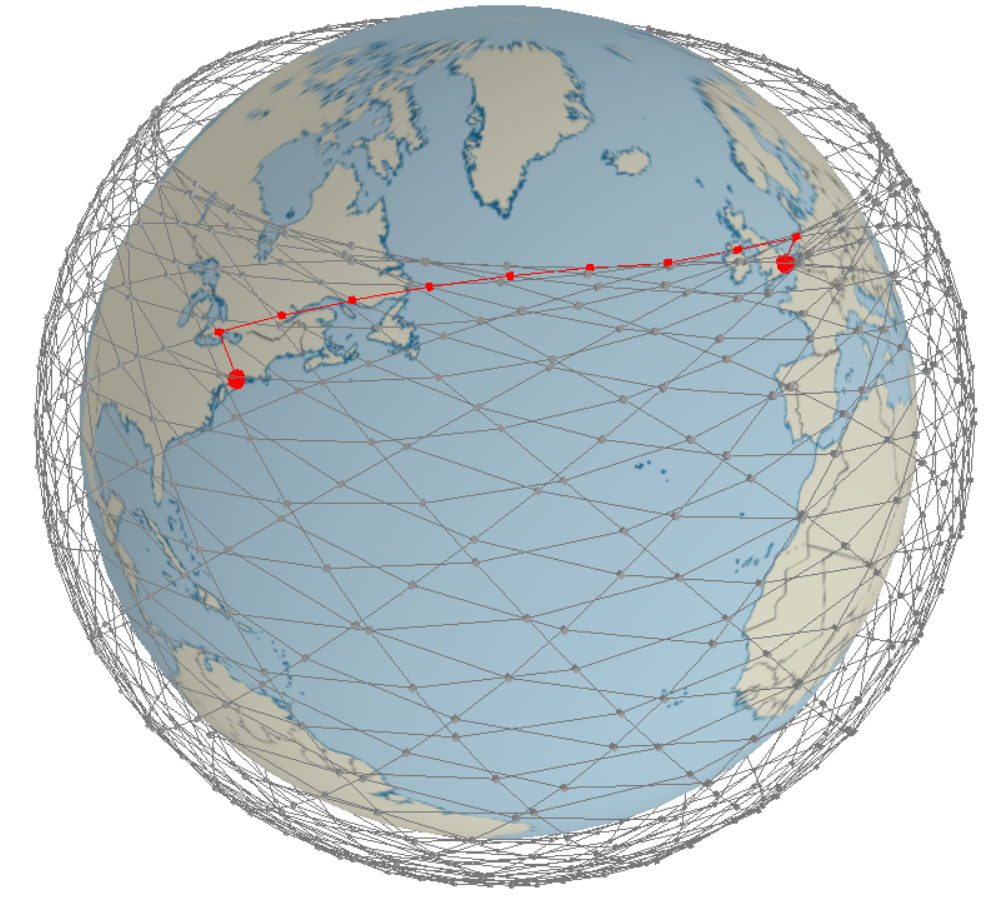
\includegraphics[width=\textwidth]{LDN-NY-H-1-1}
	\end{subfigure}
	\hfill
	\begin{subfigure}[b]{0.4\textwidth}
		\caption{The same simulation a few minutes later, now with a path that goes across the south-east moving satellites}
		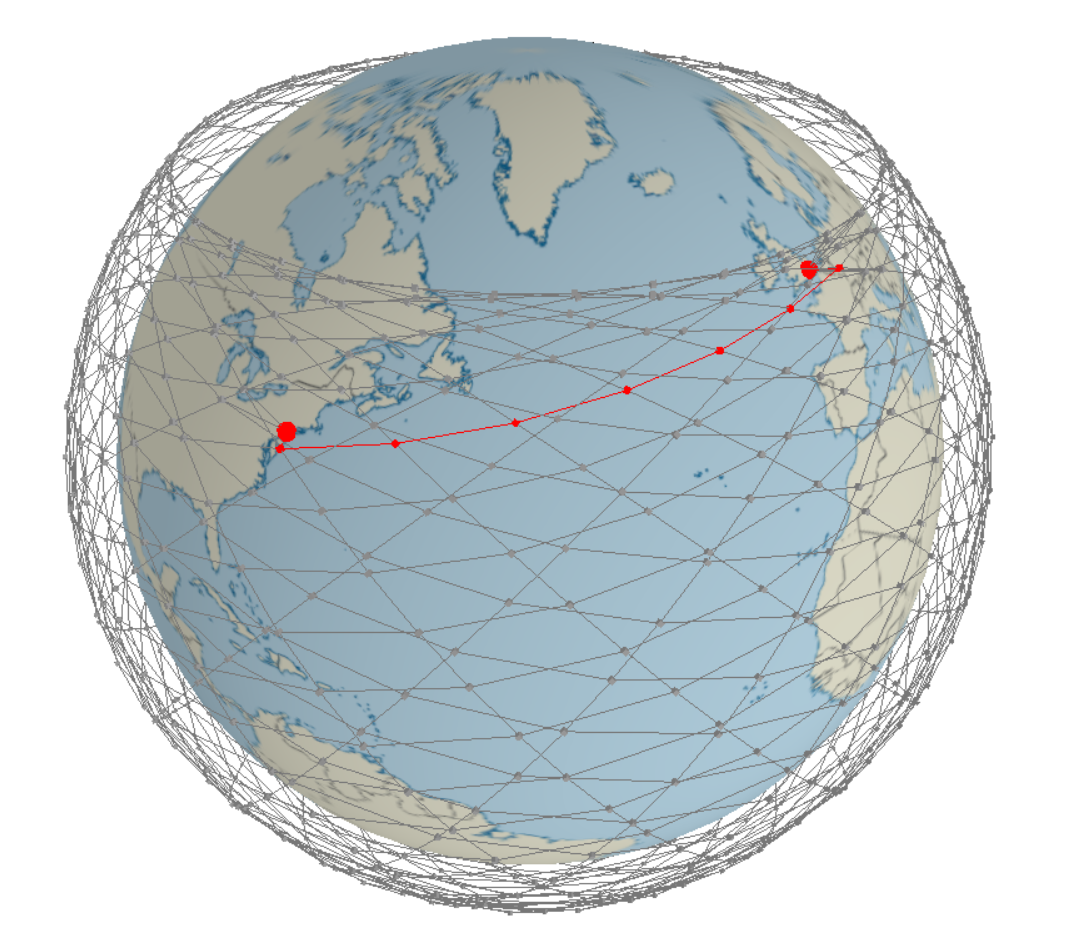
\includegraphics[width=\textwidth]{LDN-NY-H-1-2}
	\end{subfigure}
\end{figure}


%-----------------------------------------------------------------------------PERIODICITY IN LATENCIES------------------------------------------------------------------------------------
\subsection{Periodicity in Latencies}

When initially examining latencies in the network I noticed a slow transition in the result that appeared to suggest some kind of periodicity (figure \ref{fig:Latency London To New York}). To examine this further, I did a further test, this time running the model for a much longer time (figure \ref{fig:Latency London To New York Extended}). What I found was a periodicity in the latency data of almost exactly one hour. I connected this to the rotation of the earth under the Starlink network, which has 24 orbits. To confirm this I ran a third test with the Earth frozen, and found the gradual changes observed initially has disappeared (figure \ref{fig:Latency London To New York (Not Accounting for Rotation of Earth)}). As far as I can tell, this hour-long variation in the latency of a path is not something that Mark Handley accounted for in his research, however to account for it in mine, all latency results for a link will be determined by taking the average of regular samples across an hour of simulated time.

\begin{figure}
\caption{The Latency of the London-New York connection over time (extended)}
\label{fig:Latency London To New York Extended}
\begin{tikzpicture}
\begin{axis} [width=\textwidth, height=\axisdefaultheight,  xlabel={Time (minutes)}, ylabel={RTT (milliseconds)}]
\addplot table [x=Time (minutes) ,y expr=\thisrow{Time of Signal (milliseconds)} * 2, col sep=comma] {./Data/LondonToNewYorkAccelerated.csv};
\end{axis}
\end{tikzpicture}
\end{figure}

\begin{figure}
\caption{The Latency of the London-New York connection over time when the earth is treats as stationary}
\label{fig:Latency London To New York (Not Accounting for Rotation of Earth)}
\begin{tikzpicture}
\begin{axis} [width=\textwidth, height=\axisdefaultheight,  xlabel={Time (minutes)}, ylabel={RTT (milliseconds)}] 
\addplot table [x=Time (minutes), y expr=\thisrow{Time of Signal (milliseconds)} * 2, col sep=comma] {./Data/LondonToNewYorkFrozenEarth.csv};
\end{axis}
\end{tikzpicture}
\end{figure}

%============================================SELECTING MY THREE LINKING METHODS======================================================

\section{Selecting my Three Linking Methods}

Having got my tests working, my linking operational and having made some preliminary observations I could move on to choosing the three linking methods that I would examine. I chose the following three linking methods.

\begin{itemize}
\item
\[\begin{bmatrix} 
1 & 0 \\
0 & 1 
\end{bmatrix} = Handley(0)\]
\item
\[\begin{bmatrix} 
1 & -1 \\
0 & 1 
\end{bmatrix} = Handley(-1)\]
\item
\[\begin{bmatrix} 
2 & 1 \\
-1 & -1 
\end{bmatrix} = DistantLinking\]
\end{itemize}

The first two were relatively obvious picks, they were both examined by Mark Handley and I wanted the opportunity to replicate his results.

DistantLinking came from my observations of the network, I notices that satellites could comfortably connect with each other over distances much greater than just a single orbit, doing this would reduce the total hop count, and because of the spherical nature of the network, this would quite literally cut corners and reduce the overall distance.

However, there is a problem with this approach. If I chose the linking method 

\[\begin{bmatrix} 
1 & 0 \\
0 & 2 
\end{bmatrix} \]

So that each satellite connected to the satellites directly in front of, behind, and two orbits to the left and right, the resultant network would in fact be two completely disconnected components, one network of all the even numbered orbits, and one of all the odd numbered orbits. The network splitting into connected components was common whenever I tried a more complex linking than simply Handley(x). DistantLinking was one of the few linking methods I found that created both long links and remained as one connected component.

In figure \ref{fig:LMS} I show what these linking methods look like in my visualization. In DistantLinking, it is somewhat hard to see what is going on, so I recolored the constellation so that the southward moving satellites were black and the northward moving satellites were white. This can be seen in figure \ref{fig:DistantLinking}.

\begin{figure}
	\centering
	\caption{Images of the three linking methods that I examined}
	\label{fig:LMS}
	\begin{subfigure}[b]{0.3\textwidth}
		\caption{Handley(-1).}
		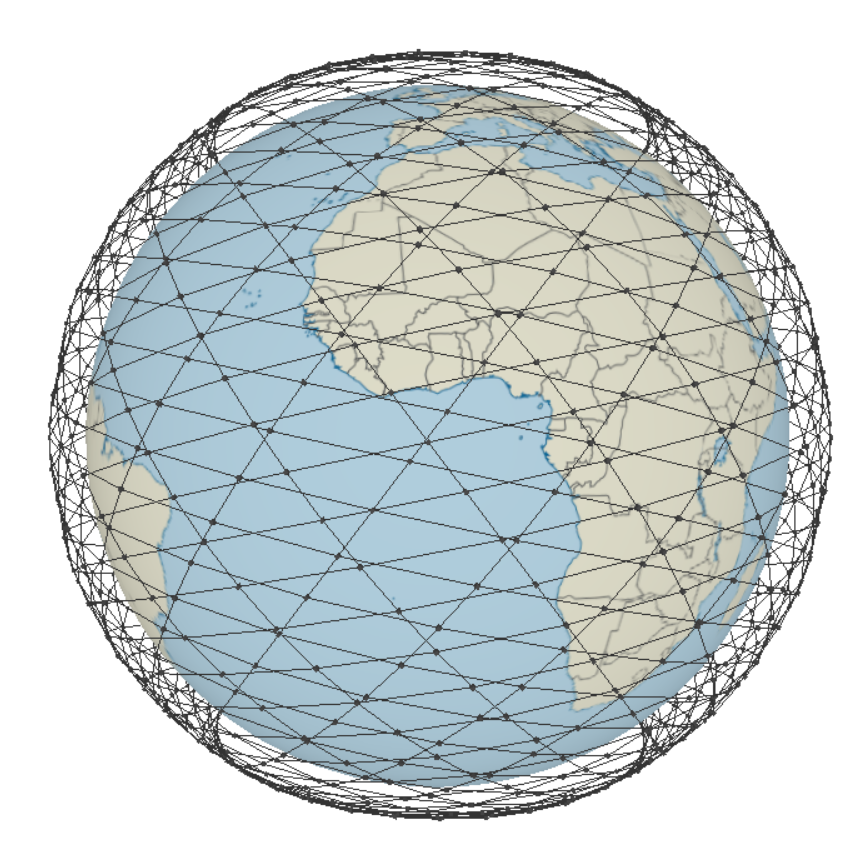
\includegraphics[width=\textwidth]{Handley-1}
	\end{subfigure}
	\hfill
	\begin{subfigure}[b]{0.3\textwidth}
		\caption{Handley(0).}
		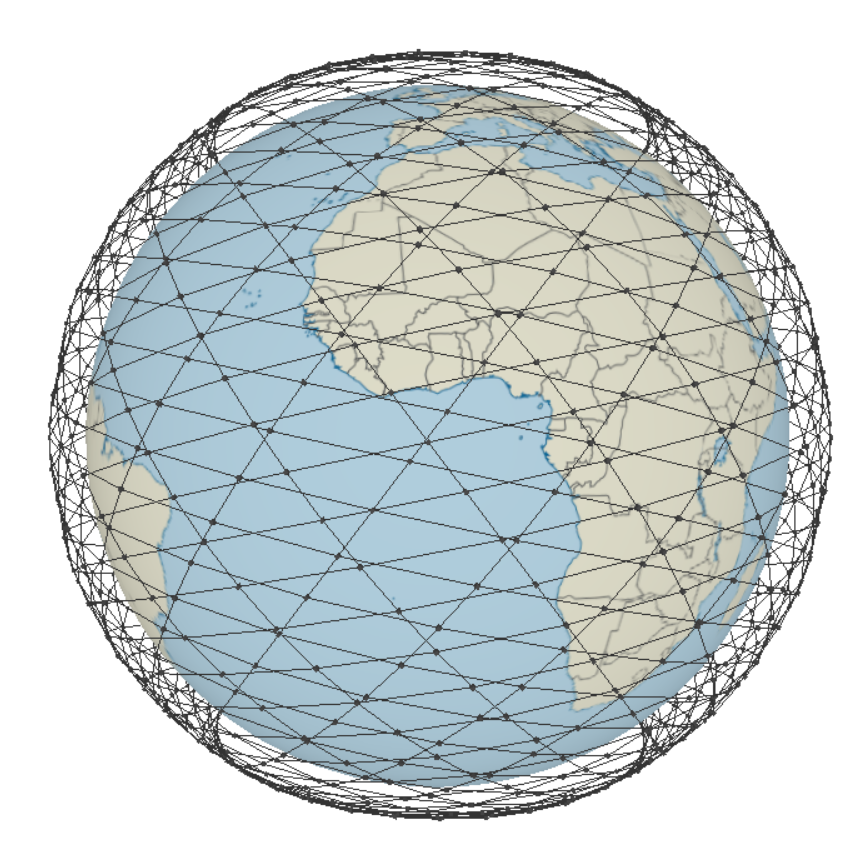
\includegraphics[width=\textwidth]{Handley-1}
	\end{subfigure}
	\hfill
	\begin{subfigure}[b]{0.3\textwidth}
		\caption{DistantLinking}
		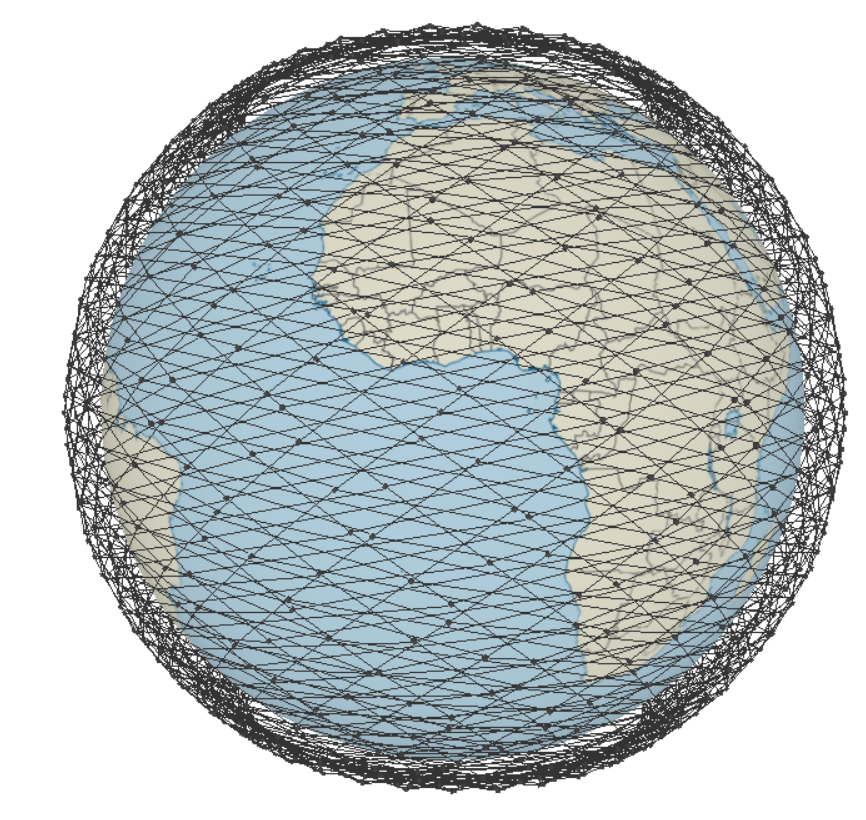
\includegraphics[width=\textwidth]{DistantLinking}
	\end{subfigure}
\end{figure}


\begin{figure}
	\centering
	\caption{DistantLinking with southward moving and northward moving satellites seperated}
	\label{fig:DistantLinking}
	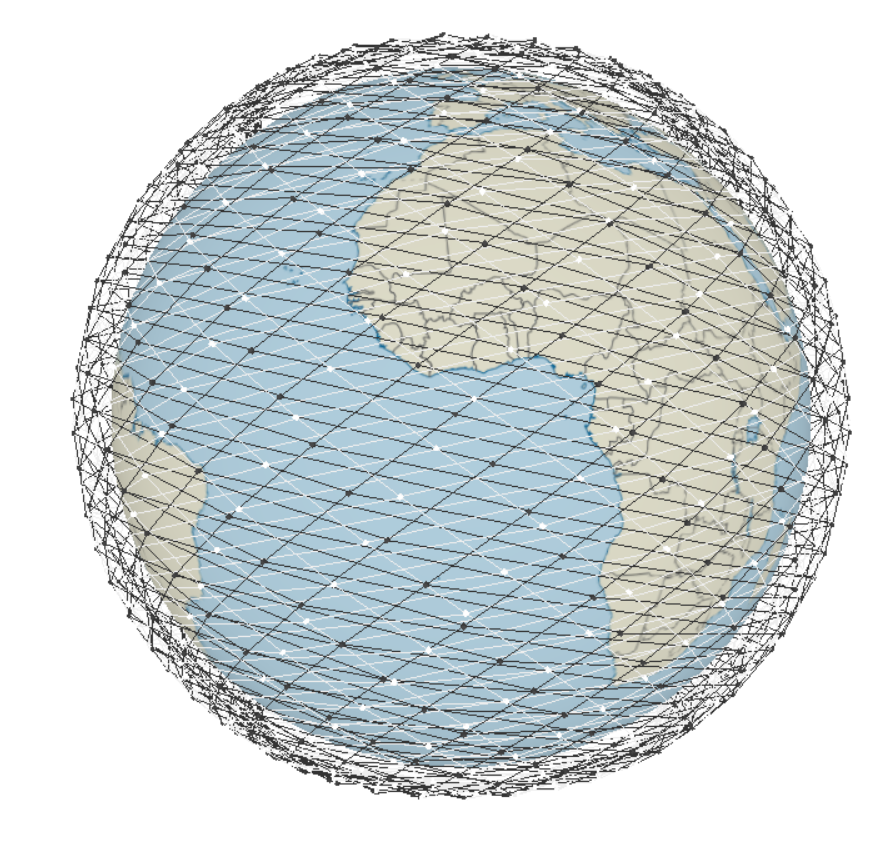
\includegraphics[width=\textwidth]{DistantLinking2}
\end{figure}

With my three linking methods chosen I could move on to examining their properties and latencies.

%==============================================================================================================================
%----------------------------------------------------------------------------------------------------------EVALUATION----------------------------------------------------------------------------------------------------------
%==============================================================================================================================
\chapter{Evaluation}

My goals going into this project were:

\begin{itemize}
\item To develop multiple routing algorithms for this network.
\item To compare these algorithms on latency, fault tolerance, and response to high demand.
\item To create visualizations of these routing algorithms at work.
\end{itemize}

With success being determined if I can test three different algorithms, producing meaningful data about their latency, fault tolerance, and response under high demand along with informative visualizations of their operations. 

It became apparent early on that "routing algorithms" was a very ambiguous term. It is not clear how one would develop an entirely new routing algorithm to operate on this network, or whether SpaceX would choose to. Furthermore, the behavior of the network is extremely predictable, which means that a base station can easily calculate the optimal path across the network and send a packet up with the exact satellites it needs to be passed between, this makes static routing the most likely option. What is very much undetermined is the topology of the network being routed across, specifically the linking method and the phase offset. Because of that, I chose to examine the properties of 3 linking methods instead.

%============================================DEVELOPING LINKING METHODS FOR THE NETWORK============================================
As stared earlier, the three linking methods I chose to examine are:

\begin{itemize}
\item Handley(0)
\item Handley(-1)
\item DistantLinking
\end{itemize}

In order to describe these linking methods I have had to create my own notation and methods of describing networks that as far as I can tell from my research have not been created before. Because of that I feel that I have achieved this goal.

%============================================COMPARING LINKING METHODS============================================
\section{Comparing Linking Methods}

%-----------------------------------------------------------------------------COMPARING LINKING METHODS ON LATENCY------------------------------------------------------------------------------------
\subsection{Comparing Linking Methods On Latency}

As outlined in the figure below \ref{fig:Linking Methods and Paths vs Failure Rate} I took three different paths that I believed tested my linking methods in different ways, London to New York (LDN-NY) was a relatively short range link between two cities at similar latitudes. New York to Beijing (BJ - NY) was a very long-range link between similar latitudes, and London - Johannesburg was a link between two very different latitudes. I then tasted the average latency over an hour for all three of my networks. My results can bee seen in figure \ref{fig:Latencies}. What I found was that Handley(-1) was superior to the other linking methods in all respects, while the DistantLinking was inferior over all three paths. The most notable exception to this was in the very long range NY-BJ path, here all three linking methods had very similar values, I speculate that this is because at an increased distance there is such a wide availability of different paths to choose from that each linking method can choose a path close to the minimum.

The results here are similar to those that Mark Handley was able to achieve in his research, and just like Mark Handley's research, my results show round trip times far shorter than anything currently available terrestrially. 

\begin{figure}
\begin{center}
\caption{The RTT of each Linking Method when there have been no satellite failures.}
\label{fig:Latencies}
\begin{tabular}{ | c | c  | c  | c |}
	\hline
	& London - New York & New York - Beijing & London - Johannesburg \\
	\hline
	Current\cite{Pings} & 75.40ms & 198,96ms\footnotemark & 163.60ms\\
	Handley(-1) & 45.94ms & 97.9ms & 105.81ms\\
	Handley(0) & 46.04ms & 97.89ms & 134.73ms\\
	DistantLinking  & 87.47ms & 103.4ms & 211.37ms\\
	\hline
\end{tabular}
\end{center}
\end{figure}

The poor performance of DistL was really surprising to me so I took to the visualization to examine why this was the case. Figure \ref{fig:Screenshots of DistL} shows why this is the case, while short paths of the form I would have hoped did appear occasionally, a great number of times DistL produced paths that were confusing at best.

Another result from my latencies was the relatively poor performance of the London-Johannesburg connection, this is a result that Handley replicated in his research, and is caused by the fact that paths between London and Johannesburg become doglegged, as seen in figure \ref{fig:Screenshots of LDN-JHB}.

\footnotetext{Unfortunately after collecting my data, I discovered that it was very challenging to find the RTT between New York and Beijing, because of this I have had to use the RTT to Seoul instead, which will be comparable but not perfect.}

\begin{figure}
	\centering
	\caption{Screenshots of DistL creating extremely long links between locations}
	\label{fig:Screenshots of DistL}
	\begin{subfigure}[b]{0.4\textwidth}
		\caption{London - New York: A path routing across the other side of the Earth}
		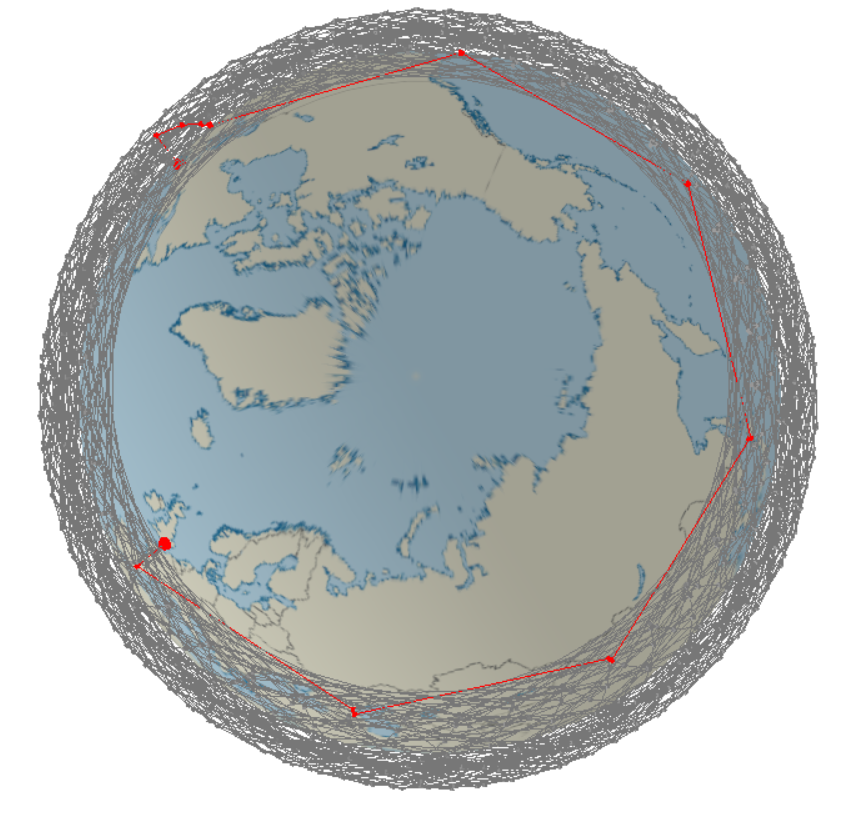
\includegraphics[width=\textwidth]{LDN-NY-DISTL-1}
	\end{subfigure}
	\hfill
	\begin{subfigure}[b]{0.4\textwidth}
		\caption{London - New York: A short path that appears only occasionally}
		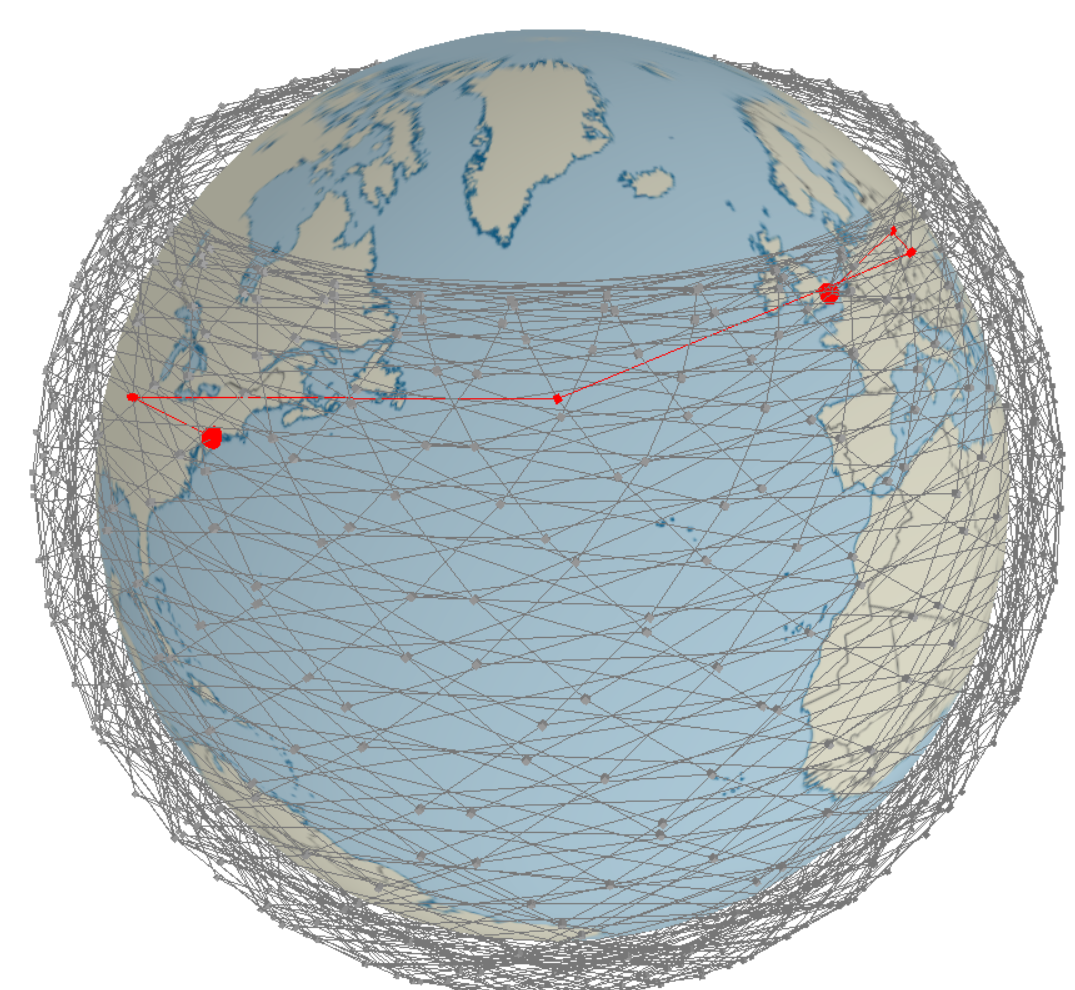
\includegraphics[width=\textwidth]{LDN-NY-DISTL-2}
	\end{subfigure}
	
	\begin{subfigure}[b]{\textwidth}
		\caption{Beijing - New York: A path with an unusal fold}
		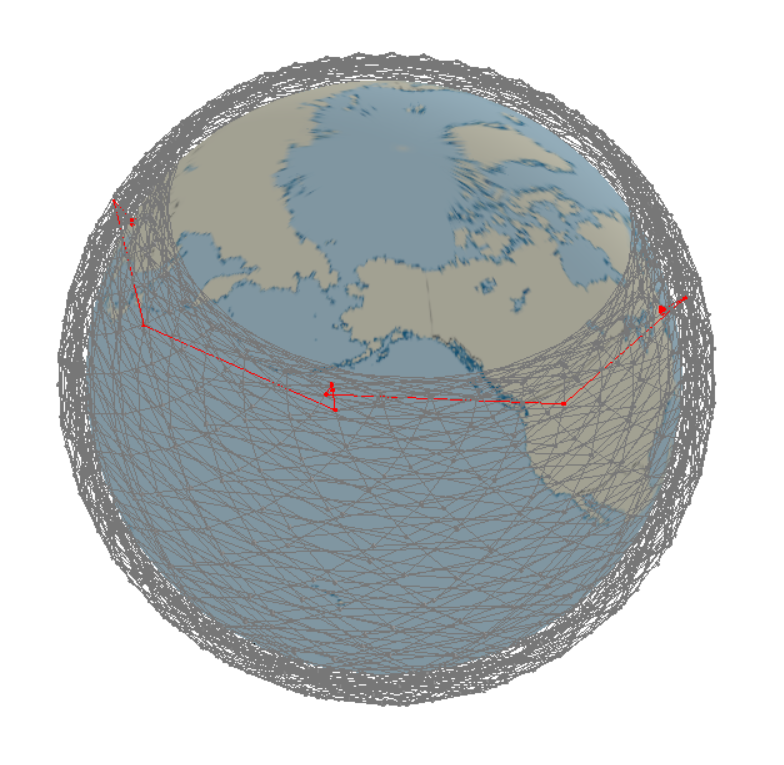
\includegraphics[width=\textwidth]{NY-BJ-DistL-1}
	\end{subfigure}
\end{figure}


\begin{figure}
	\centering
	\caption{London - Johannesburg path under different linking methods}
	\label{fig:Screenshots of LDN-JHB}
	\begin{subfigure}[b]{0.4\textwidth}
		\caption{Handley(-1)}
		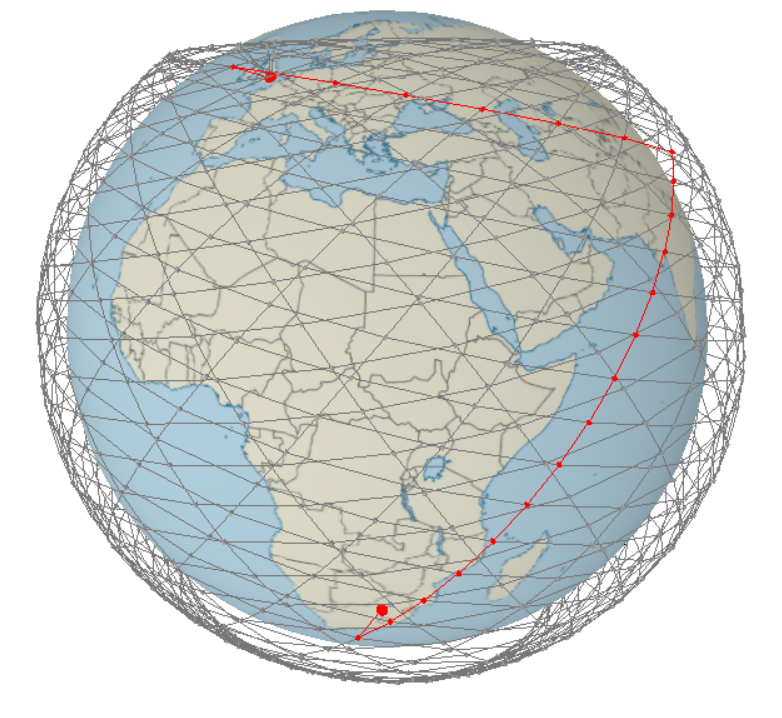
\includegraphics[width=\textwidth]{LDN-JHB-H-1-1}
	\end{subfigure}
	\hfill
	\begin{subfigure}[b]{0.4\textwidth}
		\caption{Handley(0)}
		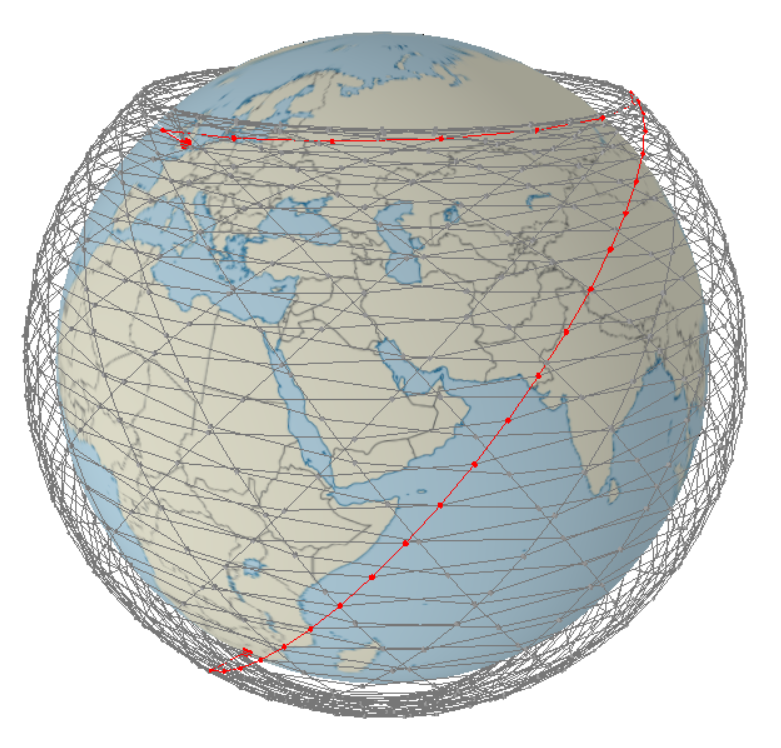
\includegraphics[width=\textwidth]{LDN-JHB-H0-1}
	\end{subfigure}
	
	\begin{subfigure}[b]{0.4\textwidth}
		\caption{DistantLinking: A very complex path}
		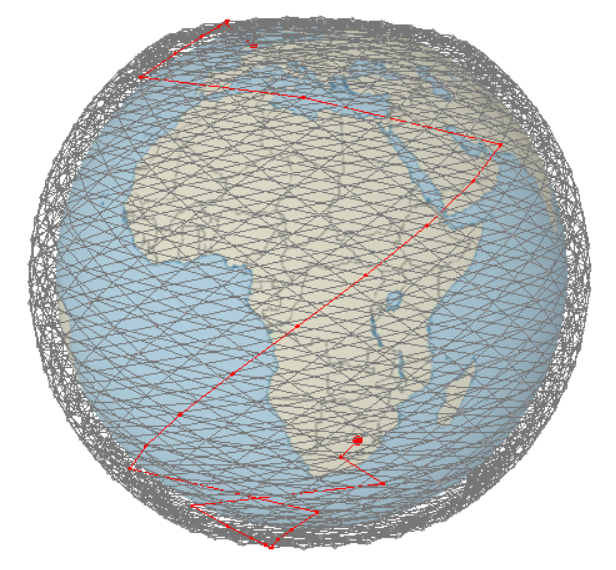
\includegraphics[width=\textwidth]{LDN-JHB-DistL-1}
	\end{subfigure}
	\hfill
	\begin{subfigure}[b]{0.4\textwidth}
		\caption{DstantLinking: A path across the other side of the world}
		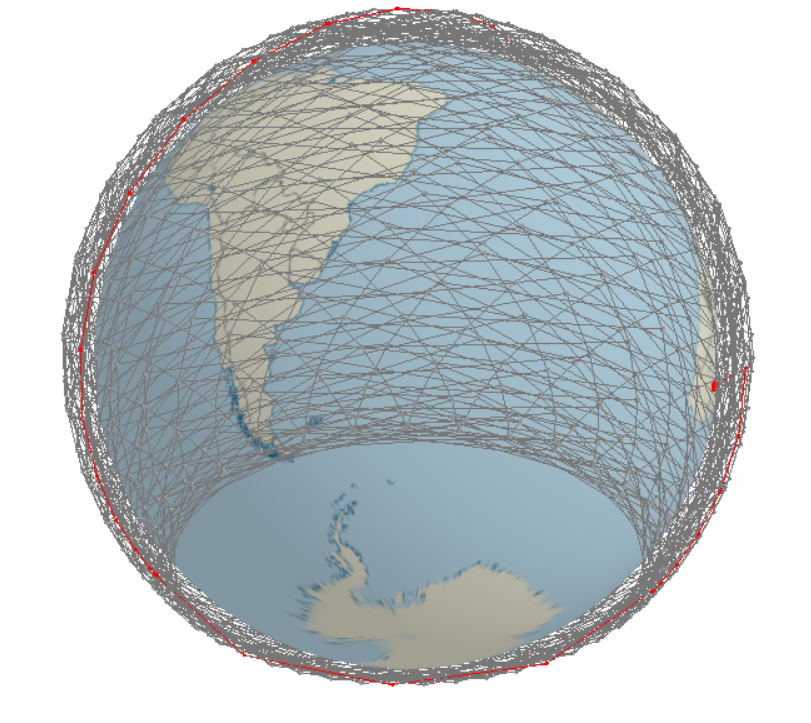
\includegraphics[width=\textwidth]{LDN-JHB-DistL-2}
	\end{subfigure}
\end{figure}

%-----------------------------------------------------------------------------COMPARING LINKING METHODS ON FAULT TOLERANCE------------------------------------------------------------------------------------
\subsection{Comparing Linking Methods On Fault Tolerance}

The first test I did for fault tolerance was a simple test of total connectivity. I deleted a certain percentage of satellites from each linking method, and then tested the total number of connected components. I did this 100 times, so that my 95\% confidence interval never exceeded 4 components. What I found is that all 3 linking methods had exactly the same curve of connected components, with the expected umber of connected components rising after a 20\% failure rate, peaking at an 80\% failure rate, and than dropping off as the number of satellites being removed from the constellation outpaced the number of new constellations being crates. This makes intuitive sense, topologically the three linking methods are all grids with the same number of elements, and so it makes sense that they would behave in the same way.

\begin{figure}
	\caption{The number of connected components after various amounts of deletion of random satellites, using the three linking methods outlined.}
	\label{fig:Connected Components After Deletions}
	\begin{tikzpicture}
		\begin{axis}  [ xlabel={Proportion of Satellites Failed}, ylabel={Average Number of Connected Components}, legend pos = north west]
			\addplot +[mark=, error bars/.cd, y dir = both, y explicit] table [x=FaliureRate, y=ConnectedComponents, col sep=comma, y error = Error] {./Data/ConnectedComponentsLM1 - Results.csv};
			\addlegendentry{Handley(-1)}
			\addplot +[mark=, error bars/.cd, y dir = both, y explicit] table [x=FaliureRate, y=ConnectedComponents, col sep=comma, y error = Error] {./Data/ConnectedComponentsLM2 - Results.csv};
			\addlegendentry{Handley(0)}
			\addplot +[mark=, error bars/.cd, y dir = both, y explicit] table [x=FaliureRate, y=ConnectedComponents, col sep=comma, y error = Error] {./Data/ConnectedComponentsLM3 - Results.csv};
			\addlegendentry{DistantLinking}
		\end{axis}
	\end{tikzpicture}
\end{figure}

To continue my examination into fault tolerance, I ran 5 hour-long tests of latency for each linking method, path, and proportion of satellites failed (in increments of 1/24ths). I took the average and then used the standard deviation to calculate 95\% confidence intervals. 

As more satellites failed, there began to be increasing amounts of "downtime" in which a path could not be established between the two ground stations. I have ignored these values when calculating path latency, but I have reflected this by including keeping track of the proportion of time that a path is available.

There are a huge number of interesting observations that can be made from this data.

First, all three linking methods and all 3 routes have a similar general behavior. As the failure rate of satellites increases, the RTT steadily increases, while the proportion of time that the link is available steadily falls. When, at around 45\% (where the average number of connected components is increasing fastest) there is a sudden drop off in the proportion of time that a link is available. After this point, for a majority of the time, there is no link between the two cities. When there is, however, this link is significantly shorter. This doesn't mean that the network has spontaneously gotten better at routing with less satellites, it just means that a steady connection between the two cities is so rare that on the few occasions it is formed, it ends to be more simple.

Another interesting observation that can be made is that the LDN-JHB link is never at 100\% availability. This is because Johannesburg is at a latitude such that between certain times of the hour there is no satellite above is that can be connected to even without any failures. This is a trait shared by all cities closer to the equator, and poses a significant limitation on the SpaceX network.

As to be expected, LDN-NY, which is a shorter path, was generally more fault tolerant than the longer BJ-NY and LDN-JHB paths. However, as seen in \ref{fig:Proportion of Time Available By Linking Method} there is no difference between the three linking methods when it comes to how they respond to failures. All this together suggests that there is no static linking method that will be any more resistant to faults in the network as these are.

All together, these results suggest the critical value for Starlink, a failure rate after which the network will be unable to function properly, is nearly 40\%. This is a very high value. Starlink claims it's satellites will have a lifespan of many years, which means that such a failure rate is extremely unlikely to occur. 

Some images of the staggered paths and disconnected networks formed at various failure rates can be seen in Figure \ref{fig:Screenshots of Failure Rate}.

\begin{figure}
	\centering
	\caption{The RTT and up time of various paths under each linking method.}
	\label{fig:Linking Methods and Paths vs Failure Rate}
	\begin{subfigure}[b]{0.3\textwidth}
		\caption{LDN - NY: H(-1)}
		\centering
		\resizebox{\textwidth}{!}{
			\begin{tikzpicture}
				\begin{axis}  [ xlabel={Proportion of Satellites Failed}, ylabel={RTT (ms)}, legend pos = north west, xmin = 0, xmax = 1, axis y line*=left]
					\addplot +[mark=, color = black, error bars/.cd, y dir = both, y explicit] table [x=FaliureRate, y=AveragePathLength, col sep=comma, y error = Error] {./Data/LondonNewYork1.csv};
				\end{axis}
				\begin{axis}  [ xlabel={Proportion of Satellites Failed}, ylabel={Proprtion of Time Path is Available}, legend pos = north west, color=blue, axis y line*=right, xmin = 0, xmax = 1, axis x line=none, ymin = 0, ymax = 1]
					\addplot +[mark=, error bars/.cd, y dir = both, y explicit] table [x=FaliureRate, y expr=1 - \thisrow{DownTime}, col sep=comma] {./Data/LondonNewYork1.csv};
				\end{axis}
			\end{tikzpicture}
		}
	\end{subfigure}
	\begin{subfigure}[b]{0.3\textwidth}
		\caption{LDN - NY: H(0)}
		\centering
		\resizebox{\textwidth}{!}{
			\begin{tikzpicture}
				\begin{axis}  [ xlabel={Proportion of Satellites Failed}, ylabel={RTT (ms)}, legend pos = north west, xmin = 0, xmax = 1, axis y line*=left]
					\addplot +[mark=, color = black, error bars/.cd, y dir = both, y explicit] table [x=FaliureRate, y=AveragePathLength, col sep=comma, y error = Error] {./Data/LondonNewYork2.csv};
				\end{axis}
				\begin{axis}  [ xlabel={Proportion of Satellites Failed}, ylabel={Proprtion of Time Path is Available}, legend pos = north west, color=blue, axis y line*=right, xmin = 0, xmax = 1, axis x line=none, ymin = 0, ymax = 1]
					\addplot +[mark=, error bars/.cd, y dir = both, y explicit] table [x=FaliureRate, y expr=1 - \thisrow{DownTime}, col sep=comma] {./Data/LondonNewYork2.csv};
				\end{axis}
			\end{tikzpicture}
		}
	\end{subfigure}
	\begin{subfigure}[b]{0.3\textwidth}
		\caption{LDN - NY: DistL}
		\centering
		\resizebox{\textwidth}{!}{
			\begin{tikzpicture}
				\begin{axis}  [ xlabel={Proportion of Satellites Failed}, ylabel={RTT (ms)}, legend pos = north west, xmin = 0, xmax = 1, axis y line*=left]
					\addplot +[mark=, color = black, error bars/.cd, y dir = both, y explicit] table [x=FaliureRate, y=AveragePathLength, col sep=comma, y error = Error] {./Data/LondonNewYork3.csv};
				\end{axis}
				\begin{axis}  [ xlabel={Proportion of Satellites Failed}, ylabel={Proprtion of Time Path is Available}, legend pos = north west, color=blue, axis y line*=right, xmin = 0, xmax = 1, axis x line=none, ymin = 0, ymax = 1]
					\addplot +[mark=, error bars/.cd, y dir = both, y explicit] table [x=FaliureRate, y expr=1 - \thisrow{DownTime}, col sep=comma] {./Data/LondonNewYork3.csv};
				\end{axis}
			\end{tikzpicture}
		}
	\end{subfigure}

	\begin{subfigure}[b]{0.3\textwidth}
		\caption{BJ - NY: H(-1)}
		\centering
		\resizebox{\textwidth}{!}{
			\begin{tikzpicture}
				\begin{axis}  [ xlabel={Proportion of Satellites Failed}, ylabel={RTT (ms)}, legend pos = north west, xmin = 0, xmax = 1, axis y line*=left]
					\addplot +[mark=, color = black, error bars/.cd, y dir = both, y explicit] table [x=FaliureRate, y=AveragePathLength, col sep=comma, y error = Error] {./Data/NewYorkBeijing1.csv};
				\end{axis}
				\begin{axis}  [ xlabel={Proportion of Satellites Failed}, ylabel={Proprtion of Time Path is Available}, legend pos = north west, color=blue, axis y line*=right, xmin = 0, xmax = 1, axis x line=none, ymin = 0, ymax = 1]
					\addplot +[mark=, error bars/.cd, y dir = both, y explicit] table [x=FaliureRate, y expr=1 - \thisrow{DownTime}, col sep=comma] {./Data/NewYorkBeijing1.csv};
				\end{axis}
			\end{tikzpicture}
		}
	\end{subfigure}
	\begin{subfigure}[b]{0.3\textwidth}
		\caption{BJ - NY: H(0)}
		\centering
		\resizebox{\textwidth}{!}{
			\begin{tikzpicture}
				\begin{axis}  [ xlabel={Proportion of Satellites Failed}, ylabel={RTT (ms)}, legend pos = north west, xmin = 0, xmax = 1, axis y line*=left]
					\addplot +[mark=, color = black, error bars/.cd, y dir = both, y explicit] table [x=FaliureRate, y=AveragePathLength, col sep=comma, y error = Error] {./Data/NewYorkBeijing2.csv};
				\end{axis}
				\begin{axis}  [ xlabel={Proportion of Satellites Failed}, ylabel={Proprtion of Time Path is Available}, legend pos = north west, color=blue, axis y line*=right, xmin = 0, xmax = 1, axis x line=none, ymin = 0, ymax = 1]
					\addplot +[mark=, error bars/.cd, y dir = both, y explicit] table [x=FaliureRate, y expr=1 - \thisrow{DownTime}, col sep=comma] {./Data/NewYorkBeijing2.csv};
				\end{axis}
			\end{tikzpicture}
		}
	\end{subfigure}
	\begin{subfigure}[b]{0.3\textwidth}
		\caption{BJ - NY: DistL}
		\centering
		\resizebox{\textwidth}{!}{
			\begin{tikzpicture}
				\begin{axis}  [ xlabel={Proportion of Satellites Failed}, ylabel={RTT (ms)}, legend pos = north west, xmin = 0, xmax = 1, axis y line*=left]
					\addplot +[mark=, color = black, error bars/.cd, y dir = both, y explicit] table [x=FaliureRate, y=AveragePathLength, col sep=comma, y error = Error] {./Data/NewYorkBeijing3.csv};
				\end{axis}
				\begin{axis}  [ xlabel={Proportion of Satellites Failed}, ylabel={Proprtion of Time Path is Available}, legend pos = north west, color=blue, axis y line*=right, xmin = 0, xmax = 1, axis x line=none, ymin = 0, ymax = 1]
					\addplot +[mark=, error bars/.cd, y dir = both, y explicit] table [x=FaliureRate, y expr=1 - \thisrow{DownTime}, col sep=comma] {./Data/NewYorkBeijing3.csv};
				\end{axis}
			\end{tikzpicture}
		}
	\end{subfigure}

	\begin{subfigure}[b]{0.3\textwidth}
		\caption{LDN - JHB: H(-1)}
		\centering
		\resizebox{\textwidth}{!}{
			\begin{tikzpicture}
				\begin{axis}  [ xlabel={Proportion of Satellites Failed}, ylabel={RTT (ms)}, legend pos = north west, xmin = 0, xmax = 1, axis y line*=left]
					\addplot +[mark=, color = black, error bars/.cd, y dir = both, y explicit] table [x=FaliureRate, y=AveragePathLength, col sep=comma, y error = Error] {./Data/LondonJohannesburg1.csv};
				\end{axis}
				\begin{axis}  [ xlabel={Proportion of Satellites Failed}, ylabel={Proprtion of Time Path is Available}, legend pos = north west, color=blue, axis y line*=right, xmin = 0, xmax = 1, axis x line=none, ymin = 0, ymax = 1]
					\addplot +[mark=, error bars/.cd, y dir = both, y explicit] table [x=FaliureRate, y expr=1 - \thisrow{DownTime}, col sep=comma] {./Data/LondonJohannesburg1.csv};
				\end{axis}
			\end{tikzpicture}
		}
	\end{subfigure}
	\begin{subfigure}[b]{0.3\textwidth}
		\caption{LDN - JHB: H(0)}
		\centering
		\resizebox{\textwidth}{!}{
			\begin{tikzpicture}
				\begin{axis}  [ xlabel={Proportion of Satellites Failed}, ylabel={RTT (ms)}, legend pos = north west, xmin = 0, xmax = 1, axis y line*=left]
					\addplot +[mark=, color = black, error bars/.cd, y dir = both, y explicit] table [x=FaliureRate, y=AveragePathLength, col sep=comma, y error = Error] {./Data/LondonJohannesburg2.csv};
				\end{axis}
				\begin{axis}  [ xlabel={Proportion of Satellites Failed}, ylabel={Proprtion of Time Path is Available}, legend pos = north west, color=blue, axis y line*=right, xmin = 0, xmax = 1, axis x line=none, ymin = 0, ymax = 1]
					\addplot +[mark=, error bars/.cd, y dir = both, y explicit] table [x=FaliureRate, y expr=1 - \thisrow{DownTime}, col sep=comma] {./Data/LondonJohannesburg2.csv};
				\end{axis}
			\end{tikzpicture}
		}
	\end{subfigure}
	\begin{subfigure}[b]{0.3\textwidth}
		\caption{LDN - JHB: DistL}
		\centering
		\resizebox{\textwidth}{!}{
			\begin{tikzpicture}
				\begin{axis}  [ xlabel={Proportion of Satellites Failed}, ylabel={RTT (ms)}, legend pos = north west, xmin = 0, xmax = 1, axis y line*=left]
					\addplot +[mark=, color = black, error bars/.cd, y dir = both, y explicit] table [x=FaliureRate, y=AveragePathLength, col sep=comma, y error = Error] {./Data/LondonJohannesburg3.csv};
				\end{axis}
				\begin{axis}  [ xlabel={Proportion of Satellites Failed}, ylabel={Proprtion of Time Path is Available}, legend pos = north west, color=blue, axis y line*=right, xmin = 0, xmax = 1, axis x line=none, ymin = 0, ymax = 1]
					\addplot +[mark=, error bars/.cd, y dir = both, y explicit] table [x=FaliureRate, y expr=1 - \thisrow{DownTime}, col sep=comma] {./Data/LondonJohannesburg3.csv};
				\end{axis}
			\end{tikzpicture}
		}
	\end{subfigure}
\end{figure}

\begin{figure}
	\caption{The proportion of time that a link is available vs the proportion of the satellites that have failed for 3 links.}
	\label{fig:Proportion of Time Available By Linking Method}
	\begin{subfigure}[b]{0,5\textwidth}
		\centering
		\caption{London-New York.}
		\resizebox{\textwidth}{!}{
			\begin{tikzpicture}
				\begin{axis}  [ xlabel={Proportion of Satellites Failed}, ylabel={Proprtion of Time Path is Available}, xmin = 0, xmax = 1, ymin = 0, ymax = 1]
					\addplot +[mark=] table [x=FaliureRate, y expr=1 - \thisrow{DownTime}, col sep=comma] {./Data/LondonNewYork1.csv};
					\addlegendentry{Handley(-1)}
					\addplot +[mark=] table [x=FaliureRate, y expr=1 - \thisrow{DownTime}, col sep=comma] {./Data/LondonNewYork2.csv};
					\addlegendentry{Handley(0)}
					\addplot +[mark=] table [x=FaliureRate, y expr=1 - \thisrow{DownTime}, col sep=comma] {./Data/LondonNewYork3.csv};
					\addlegendentry{DistantLinking}
				\end{axis}
			\end{tikzpicture}
		}
	\end{subfigure}
	\begin{subfigure}[b]{0.5\textwidth}
		\centering
		\caption{New York-Beijing.}
		\resizebox{\textwidth}{!}{
			\begin{tikzpicture}
				\begin{axis}  [ xlabel={Proportion of Satellites Failed}, ylabel={Proprtion of Time Path is Available}, xmin = 0, xmax = 1, ymin = 0, ymax = 1]
					\addplot +[mark=] table [x=FaliureRate, y expr=1 - \thisrow{DownTime}, col sep=comma] {./Data/NewYorkBeijing1.csv};
					\addlegendentry{Handley(-1)}
					\addplot +[mark=] table [x=FaliureRate, y expr=1 - \thisrow{DownTime}, col sep=comma] {./Data/NewYorkBeijing2.csv};
					\addlegendentry{Handley(0)}
					\addplot +[mark=] table [x=FaliureRate, y expr=1 - \thisrow{DownTime}, col sep=comma] {./Data/NewYorkBeijing3.csv};
					\addlegendentry{DistantLinking}
				\end{axis}
			\end{tikzpicture}
		}
	\end{subfigure}
	\begin{subfigure}[b]{0.5\textwidth}
		\centering
		\caption{London-Johannesburg.}
		\resizebox{\textwidth}{!}{
			\begin{tikzpicture}
				\begin{axis}  [ xlabel={Proportion of Satellites Failed}, ylabel={Proprtion of Time Path is Available}, xmin = 0, xmax = 1, ymin = 0, ymax = 1]
					\addplot +[mark=] table [x=FaliureRate, y expr=1 - \thisrow{DownTime}, col sep=comma] {./Data/LondonJohannesburg1.csv};
					\addlegendentry{Handley(-1)}
					\addplot +[mark=] table [x=FaliureRate, y expr=1 - \thisrow{DownTime}, col sep=comma] {./Data/LondonJohannesburg2.csv};
					\addlegendentry{Handley(0)}
					\addplot +[mark=] table [x=FaliureRate, y expr=1 - \thisrow{DownTime}, col sep=comma] {./Data/LondonJohannesburg3.csv};
					\addlegendentry{DistantLinking}
				\end{axis}
			\end{tikzpicture}
		}
	\end{subfigure}
\end{figure}

\begin{figure}
	\centering
	\caption{Screenshots of Various Linking Methods at Different Failure Rates Responding to the failure rate}
	\label{fig:Screenshots of Failure Rate}
	\begin{subfigure}[b]{0.4\textwidth}
		\caption{NY-BJ, 70\% faliure rate}
		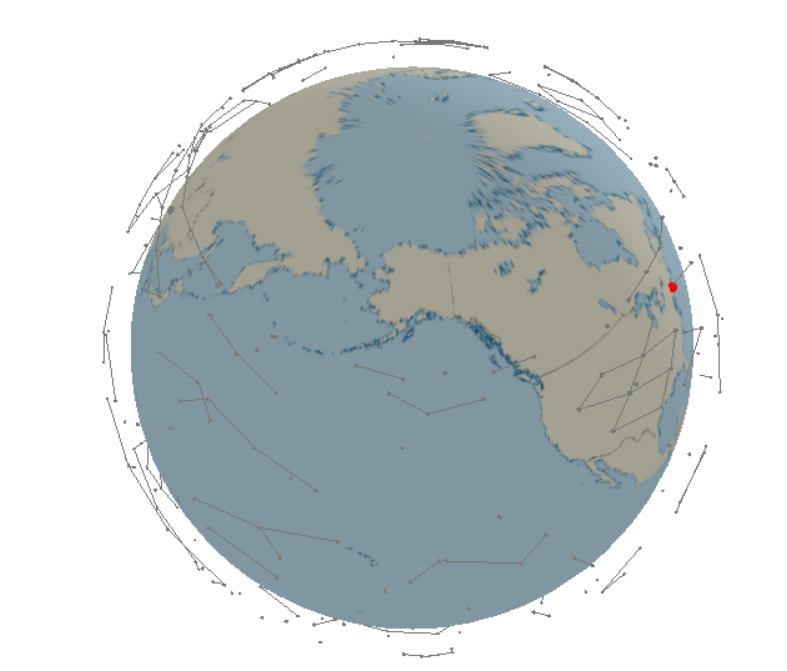
\includegraphics[width=\textwidth]{NewYorkBeijing462Satellites}
	\end{subfigure}
	\hfill
	\begin{subfigure}[b]{0.4\textwidth}
		\caption{NY-BJ, H(0), 17\% faliure rate}
		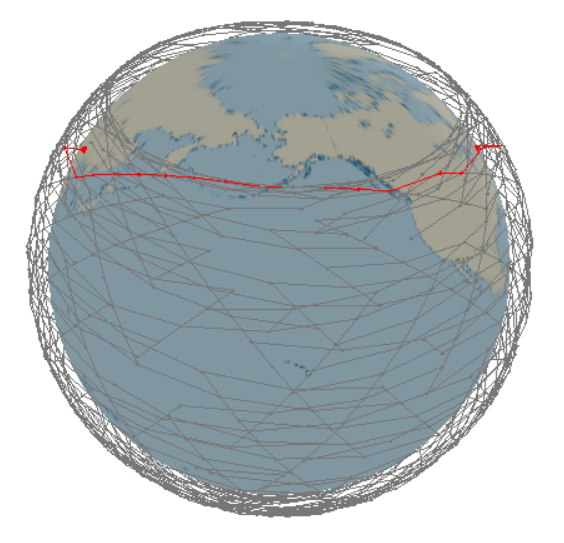
\includegraphics[width=\textwidth]{NewYorkBeijing1320SatellitesLM2}
	\end{subfigure}
	
	\begin{subfigure}[b]{\textwidth}
		\caption{LDN-JHB, H(0), 21\% faliure rate}
		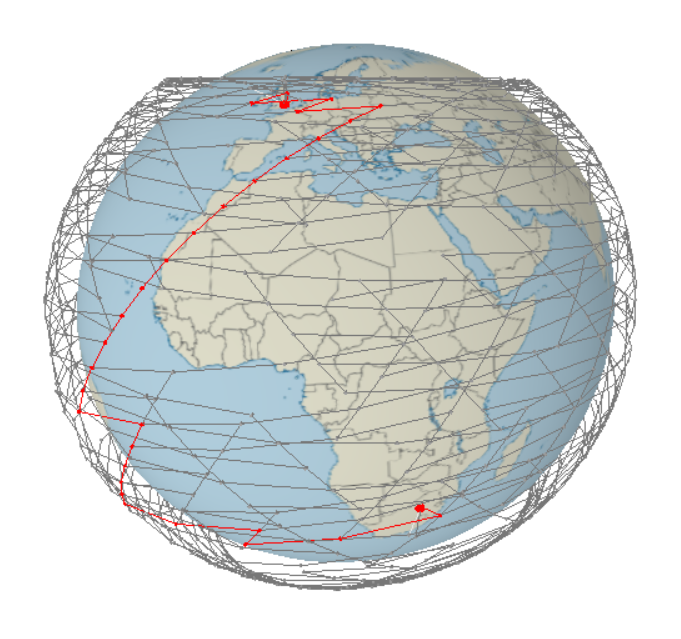
\includegraphics[width=\textwidth]{LondonJohannasburg1254SatellitesLM2}
	\end{subfigure}
\end{figure}


%-----------------------------------------------------------------------------COMPARING LINKING METHODS ON RESPONSE TO HIGH DEMAND------------------------------------------------------------------------------------

\subsection{Comparing Linking Methods On High Demand}
I did not have time to calculate n shortest paths around the network, though I believe that some knowledge about how the Linking Methods might respond to high demand can be gleaned from how they respond to satellite failure, as the ability to resist failure is connected to having multiple different ways to route between two points, which in turn is connected closely to fault tolerance. Because of this, I would expect all three linking methods to be equally effective at dealing with high demands.

%============================================VISUALISING THE LINKING METHODS AT WORK============================================

\section{Visualizing the Linking Methods at Work}

I believe that my goal of visualizing the linking methods at work has been effectively achieved through the available executable and screenshots that have been taken. By visualizing the network like this I believe that I have gained, and have the ability to give to others, and intuitive understanding for how this network works that can direct further research into it's properties, as well has having contributed to and directed my own research into it's properties.

\section{Direction and Focus}

Maintaining a consistent goal has been challenging during such an open-ended project. If I were to do this project again I would more carefully choose my objectives I believe that I made a mistake in talking about "routing algorithms" in my original proposal, as while linking methods could be considered a form of routing algorithm, these concepts are fundamentally different, and I should not have 

A number of projects in the early phrases had to be abandoned not just because of inefficiency but because new information came about that rendered them useless.

The announcement from SpaceX that they were significantly changing the constellation had massive impacts to the project. Firstly, the new satellites would have only four links instead of five, this implied that the satellites would not not have a "free" link but would instead be connected only to those ahead of and behind them. Because of this, I decided to drop the free links from my model, but doing so meant that a large chunk of code that had been written was discarded.

The knowledge that SpaceX were willing to change their designs so abruptly also had a significant impact on modeling their constellation. It is likely that the second and third phases of Starlink will be similarly changed to be in similar altitudes to phase one, however without a full understanding on what these new spheres would be, or how they would connect to phase one, it was elected to instead focus solely on the first sphere's constellation.

Overall I think that this project has been somewhat of a success, in that I have contributed in a meaningful way to a growing body of research and confirmed and supported the finding of the researchers at UCL. But because of the poor initial planning of the project I cannot call it a full success.

%==============================================================================================================================
%----------------------------------------------------------------------------------------------------------CONCLUSION---------------------------------------------------------------------------------------------------------
%==============================================================================================================================
\chapter{Conclusion}

I have shown, through examining three different linking methods, that we can expect similar fault tolerance and response to high load from any grid-like linking method that SpaceX chooses to employ, but that these linking methods vary significantly in the expected latencies. I also believe that I have shown that the linking method that SpaceX choose to do with will most likely be of the Handley(x) form, rather than anything more complex.

I also believe that I have in the process of writing this report made a number of other discoveries that will inform future research. The discovery of the 60-minute variations in latencies is in my opinion very significant, this is something that I have not seen observed in any of the research thus far but has a significant impact on how one calculates latencies across the network. The discovery that locations close the equator will not be consistently connected to the Starlink network is also very notable.

\section{Extension}

Were I to come back to this project I would do a number of things differently. I think that I have been let down by a lack of imagination in how linking methods might work, all of the linking methods I ended up choosing where fundamentally grids and therefore limited in the differences in their behavior. I would have liked to have experimented with more complex linking methods, perhaps ones that divided up satellites into two classes, one for long ranged communication and one for short ranged, creating a condensed grid. I wild also have liked to experiment with allowing satellites to respond to failures in the network, for instance by moving into a gap left behind by a failed satellite or by connecting to the satellite on he other side of the gap.

I also think that it would have been worthwhile to examine how such a network would connect to other orbital spheres. SpaceX intends to send up more spheres of satellites in the future, but how / if these spheres of satellites will interact is as of yet unknown. Modeling various ways that two spheres of satellites could communicate, especially when both spheres have only four links per satellite, would be incredibly interesting.

Building off of the data collected on the changes in path latency, I think simulations of different implementations of TCP under these kinds of latencies would be very worthwhile, to see if the variation in latencies is tolerable by TCP. And I think it would be worthwhile to simulate how TCP behaves around the sudden changes in latency created when a new path is opened up, while these changes no not happen frequently, TCP is very sensitive to packet reordering and I would be curious to know if it can handle the packet reordering caused by such a significant change in latency and if there are any protocols for path hand over that would improve this. As far as I know no such experiments have yet been done, and it is an opportunity to build off of my current work that I think would be really valuable.

\begin{thebibliography}{99}
	%using the vancouver system https://en.wikipedia.org/wiki/Vancouver_system
	\bibitem{PriorityQueue1} Daniel Pflughoeft. High Speed Priority Queue for C Sharp.
	2013. Available from:  \url{https://github.com/BlueRaja/High-Speed-Priority-Queue-for-C-Sharp}
	\bibitem{PriorityQueue2} Dr. James McCaffrey. Priority Queues with C\#. 
	Visual Studio Magazine. 2012. Available from: \url{https://visualstudiomagazine.com/Articles/2012/11/01/Priority-Queues-with-C.aspx}
	\bibitem{Pings} WonderNetwork. Global Pink Statistics. 
	Available from: \url{https://wondernetwork.com/pings}
	\bibitem{ExedeWebsite} Exede. Website.
	Available from:\url{https://www.exede.com}
	\bibitem{HughesWebsite} Hughes. Website.
	Available from: \url{https://www.hughes.com}
	\bibitem{ElonMuskTweet} Elon Musk. Twitter.
	2018. Available from: \url{https://twitter.com/elonmusk/status/1000453321121923072}
	\bibitem{ElonMuskTwee2t} Elon Musk. Twitter.
	2019. Available from: \url{https://twitter.com/elonmusk/status/1127388838362378241}
	\bibitem{FCCApplication} Federal Communications Commission (FCC). File Number = SATLOA2016111500118.
	2018. Available from: \url{licensing.fcc.gov/cgi-bin/ws.exe/prod/ib/forms/reports/related_filing.hts?f_key=-289550&f_number=SATLOA2016111500118}
	\bibitem{TechnicalAttachment} SpaceX. Attatchment A: Technical Informaton to Supplement Schedule S.
	Federal Communications Commission (FCC). 2016. Available from: \url{https://licensing.fcc.gov/myibfs/download.do?attachment_key=1158350}
	\bibitem{OriginalReport} Mark Handley. Delay is Not an Option: Low Latency Routing in Space.
	2018. University College London. Avaialble from: \url{http://nrg.cs.ucl.ac.uk/mjh/starlink/}
	\bibitem{HughesPressRelease} Hughes. Hughes High-Throughput Satellite Successfully Launched, Setting the Stage for the Next Generation of Satellite Internet.
	2016. Available From: \url{https://www.hughes.com/who-we-are/resources/press-releases/hughes-high-throughput-satellite-successfully-launched-setting?locale=en}
	\bibitem{EchoStar} Gunter's Space Page. Jupiter 2 / EchoStar19.
	2015. Available from: \url{https://space.skyrocket.de/doc_sdat/jupiter-2.htm}
	\bibitem{FirstPersonMotion} Turtletooth. Godot First Person Controller. 
	2017. Available from: \url{https://github.com/turtletooth/GodotFirstPersonController}
	\bibitem{Map} Wikipedia. USGS majplatecolor.png.
	2012.Available from: \url{https://commons.wikimedia.org/wiki/File:USGS_majplatecolor.png}
	\bibitem{Book} C.D. Murral and S.F. Dermott. Solar System Dymanics. 1999. Cambridge University Press.
	\bibitem{HowMuchJitter} VoIP Studio, VoIP And How Much Jitter Is Acceptable?
	2015, Available from: \url{https://voipstudio.com/blog/voip-how-much-jitter-is-acceptable/}
	\bibitem{StarlinkChange} Chris Davis, "As launch nears, SpaceX’s Starlink satellite internet gets big change approval"
	SlashGear, 2019, Available from: \url{https://www.slashgear.com/as-launch-nearsspacexs-starlink-satellite-internet-gets-big-change-approval-29574978/}
\end{thebibliography}
\appendix

%TODO Project Proposal

\end{document}